\chapter{Slepian Scale-Discretised Wavelets on Manifolds}\label{sec:chapter4}

\section{Introduction}

\section{Mathematical Background and Problem Formulation}

\subsection{Mathematical Preliminaries}

\subsubsection{Riemannian Manifolds}

Let \(\manifold{}\) denote a compact, smooth, connected \(d\)-dimensional Riemannian manifold without boundary contained in \(\mathbb{R}^{n}\).
The Hilbert space \(\hilbert{\manifold}\) is formed by the set of functions \(f : \manifold \to \mathbb{R}\) that are square-integrable with respect to the Riemannian volume \(\meshVolume{}\).
The geodesic distance between two points is denoted \(r(x,y)\), and the Laplace-Beltrami operator on \(\manifold{}\) is denoted \(\laplacian{}\).
Let the set of all isometries between two manifolds \(\manifold{}\) and \(\manifold'\) be denoted \(\isom{\manifold,\manifold'}\), and set \(\isom{\manifold} = \isom{\manifold,\manifold}\) to be the isometry group of \(\manifold{}\).
Similarly, \(\diff{\manifold} = \diff{\manifold,\manifold}\) is set to be the diffeomorphism group on \(\manifold{}\).

In practice, one must discretise the manifolds and represent them as graphs.
A review of graphs is presented in \cref{sec:chapter4_graphs}.

\subsubsection{Graphs}\label{sec:chapter4_graphs}

\subsubsection{Polygonal Meshes}

\begin{figure}[htp]
	\centering
	\subfloat[\(\mesh{\phi_{3}}\)]
	{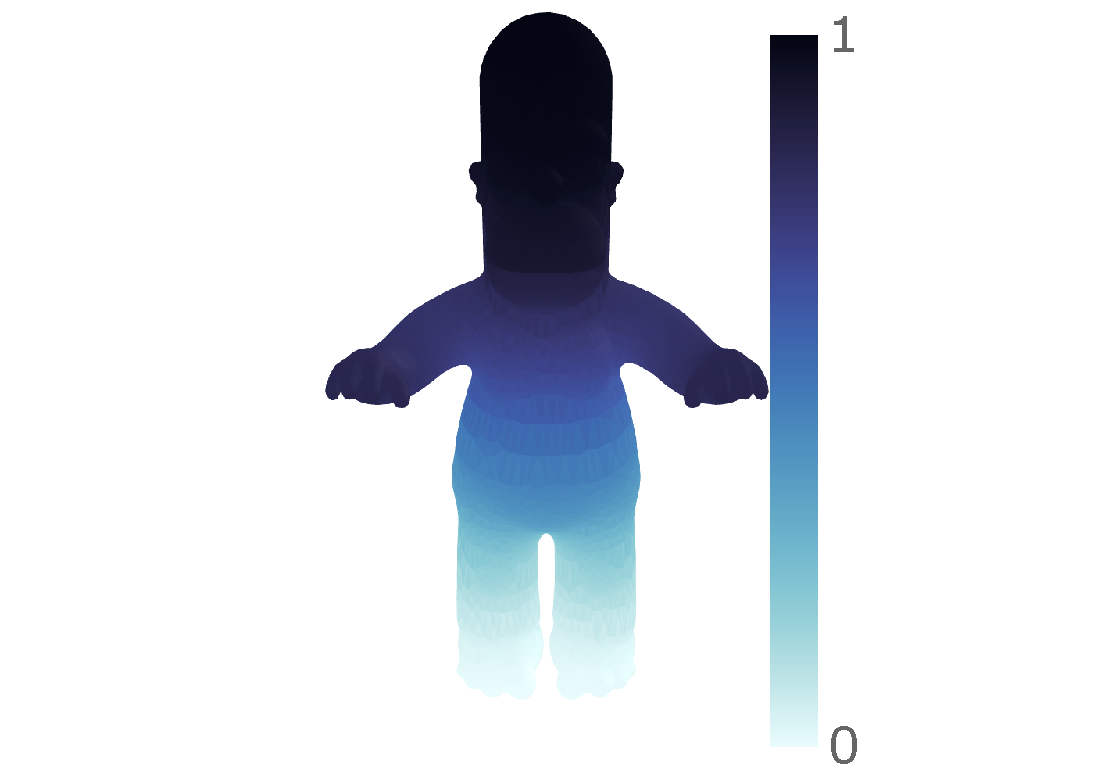
\includegraphics[trim={156 8 21 6},clip,width=.25\textwidth]{homer_rank2_lam1-325328e-03_norm.pdf}} % chktex 8
	\hfill
	\subfloat[\(\mesh{\phi_{4}}\)]
	{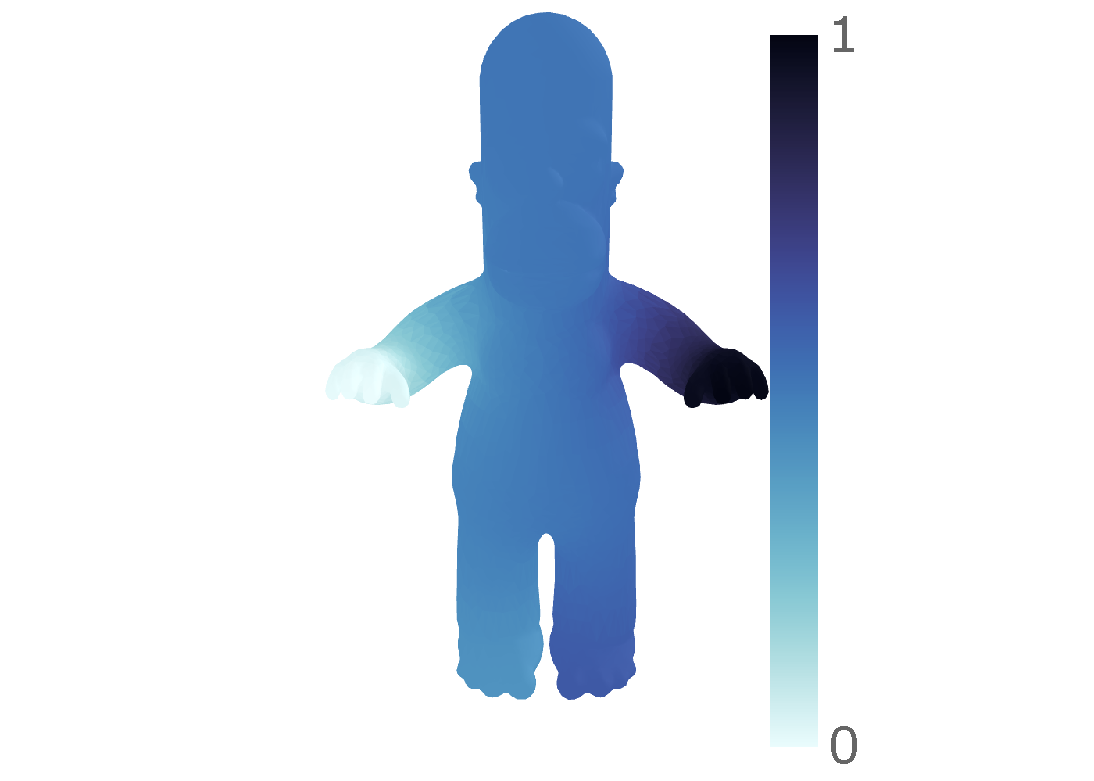
\includegraphics[trim={156 8 21 6},clip,width=.25\textwidth]{homer_rank3_lam2-425344e-03_norm.pdf}} % chktex 8
	\hfill
	\subfloat[\(\mesh{\phi_{5}}\)]
	{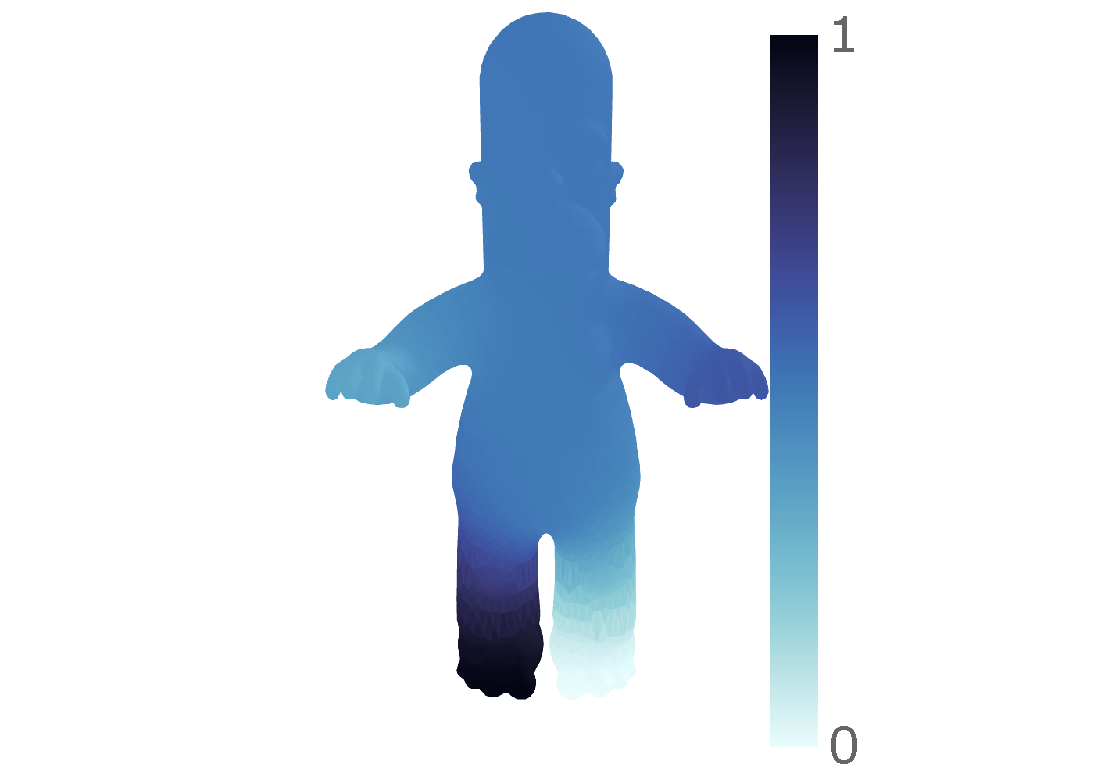
\includegraphics[trim={156 8 21 6},clip,width=.25\textwidth]{homer_rank4_lam2-706937e-03_norm.pdf}} % chktex 8
	\hfill
	\subfloat[\(\mesh{\phi_{6}}\)]
	{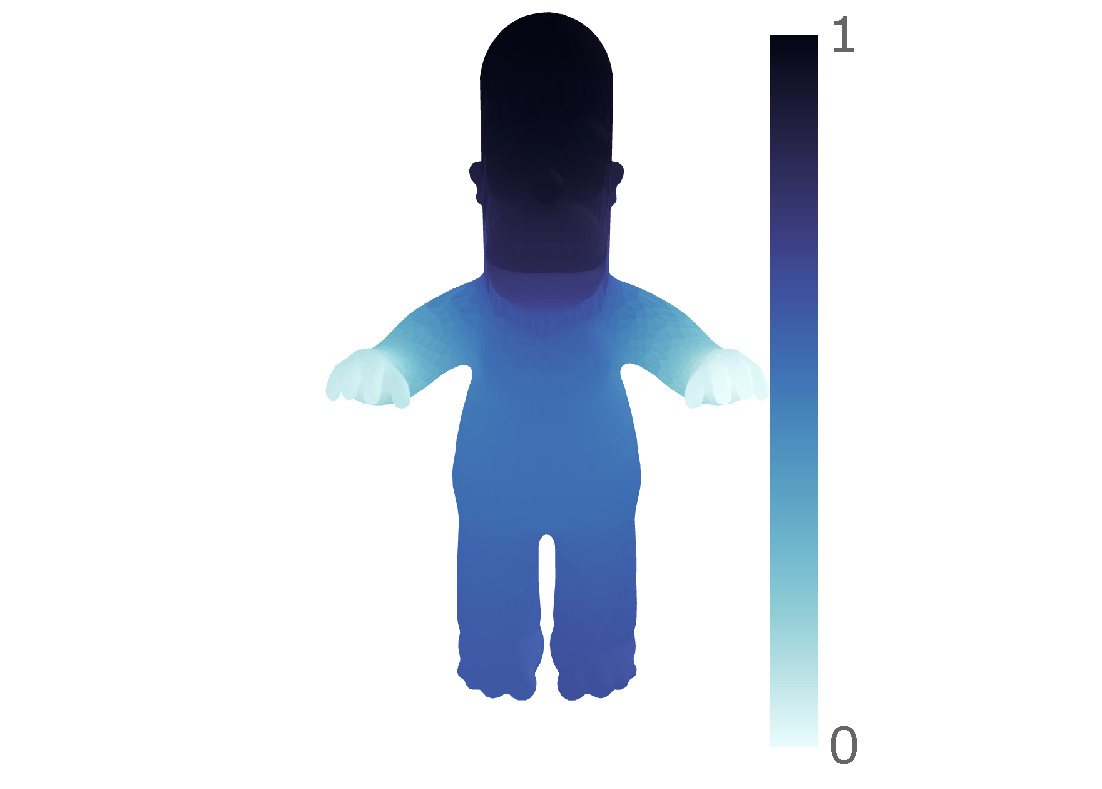
\includegraphics[trim={156 8 21 6},clip,width=.25\textwidth]{homer_rank5_lam2-851096e-03_norm.pdf}} % chktex 8
	\newline
	\subfloat[\(\mesh{\phi_{7}}\)]
	{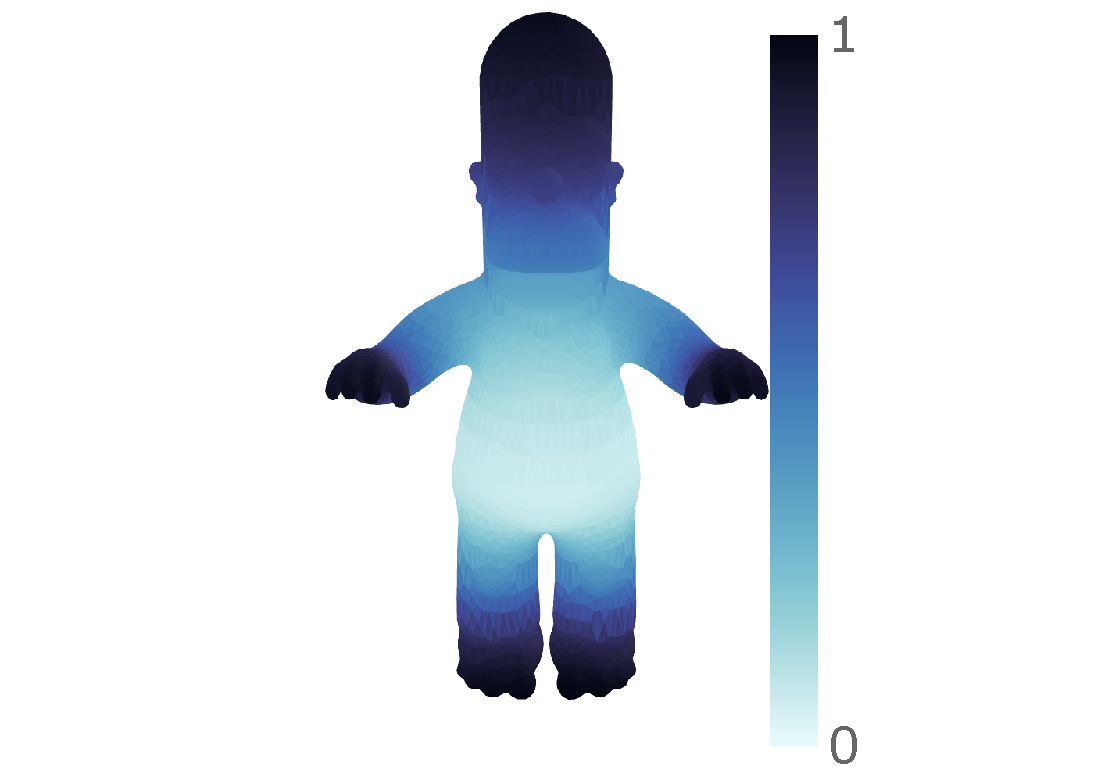
\includegraphics[trim={156 8 21 6},clip,width=.25\textwidth]{homer_rank6_lam7-806422e-03_norm.pdf}} % chktex 8
	\hfill
	\subfloat[\(\mesh{\phi_{8}}\)]
	{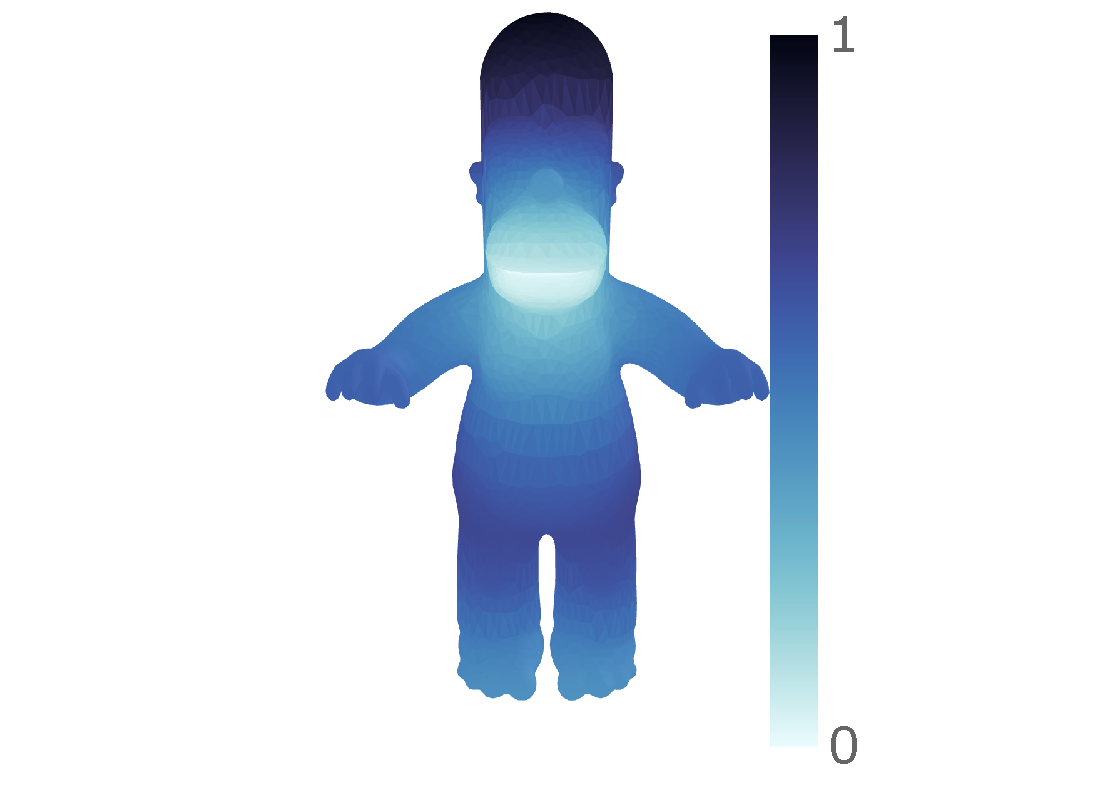
\includegraphics[trim={156 8 21 6},clip,width=.25\textwidth]{homer_rank7_lam1-164387e-02_norm.pdf}} % chktex 8
	\subfloat[\(\mesh{\phi_{9}}\)]
	{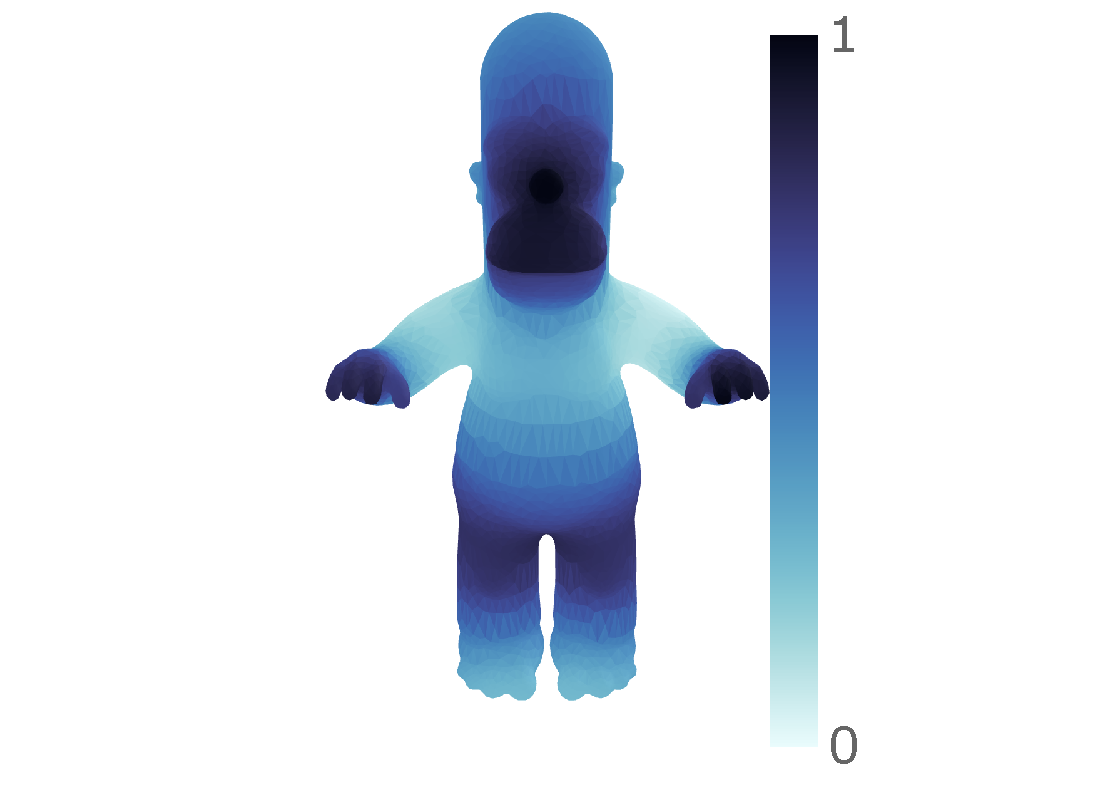
\includegraphics[trim={156 8 21 6},clip,width=.25\textwidth]{homer_rank8_lam1-738974e-02_norm.pdf}} % chktex 8
	\hfill
	\subfloat[\(\mesh{\phi_{10}}\)]
	{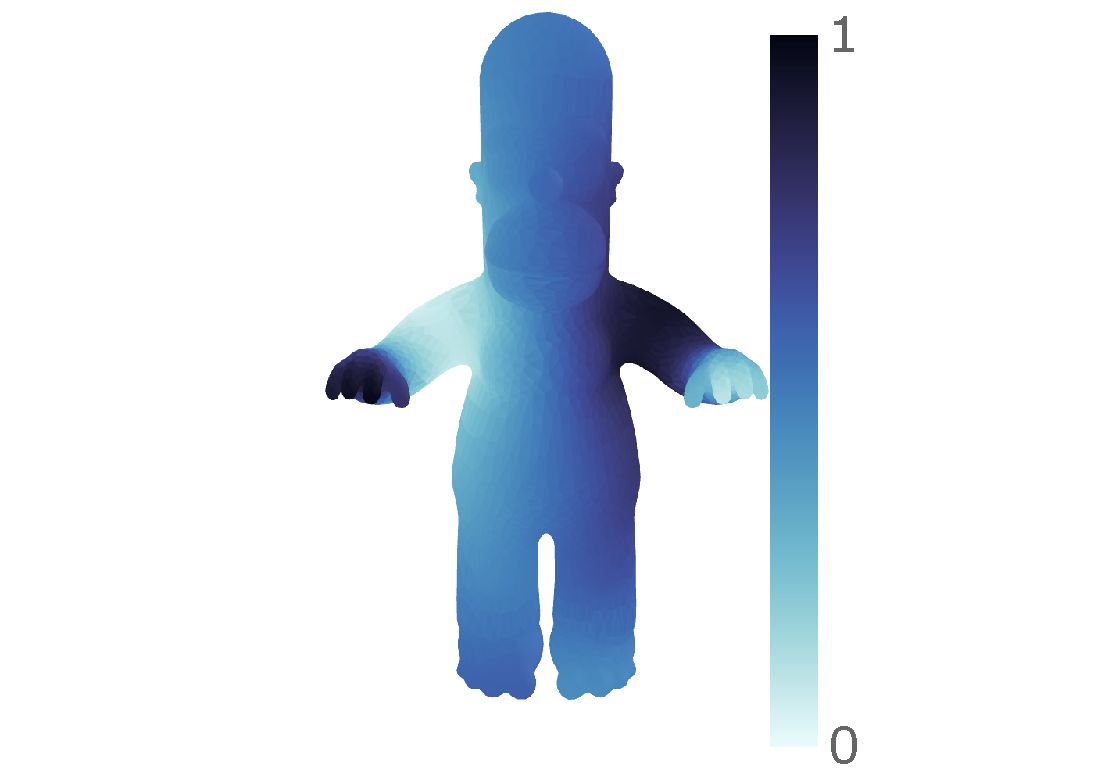
\includegraphics[trim={156 8 21 6},clip,width=.25\textwidth]{homer_rank9_lam1-827015e-02_norm.pdf}} % chktex 8
	\caption{
		The third to tenth eigenvectors of the mesh Laplacian of a Homer Simpson mesh ordered by increasing eigenvalue (frequency).
		In total \(\num{1275}\) basis functions of the \(\num{5103}\) vertex mesh were computed.
		Whilst the eigenvectors are defined on the vertices, the values have been averaged onto the faces for the plot.
	}\label{fig:chapter4_eigenhomers}
\end{figure}


\subsection{Slepian Scale-Discretised Wavelets on the Sphere}\label{sec:chapter4_slepian_scale_discretised_wavelets_sphere}

\subsection{Problem Formulation}

This work generalises Slepian scale-discretised wavelets on the sphere, defined in \cref{sec:chapter4_slepian_scale_discretised_wavelets_sphere}, to arbitrary manifolds.

\section{Working with Manifolds}

In this section a review of the Slepian spatial-spectral concentration problem is presented in \cref{sec:chapter4_slepian_concentration_problem_manifolds}.
A review of the sifting convolution follows in \cref{sec:chapter4_sifting_convolution_manifolds} which allows one to perform convolutions on manifolds.

\subsection{Slepian Concentration Problem on Manifolds}\label{sec:chapter4_slepian_concentration_problem_manifolds}

The problem of spatial concentration of bandlimited signals (likewise spectral concentration of spacelimited signals) was first studied by Slepian, Landau and Pollak in the 1960s~\cite{Slepian1961,Landau1961,Landau1962}.
Initially for time domain signals, it has since been extended to other domains such as signals on the sphere~\cite{Simons2006,Roddy2021a,Xu1983,Wieczorek2005}.
This work considers optimally concentrated functions within a region \(R\) of a manifold \(\manifold{}\), an example of which is shown in \cref{fig:chapter4_region}.

% Inspired by Fionn Fitzmaurice's differential geometry notes
% https://gist.github.com/fionn/f27ddeadba97f3dabbf97527b05b33e5
\begin{figure}[htp]
	\centering
	\resizebox{0.75\textwidth}{!}{%
		\begin{tikzpicture}
			\begin{scope}
				\draw [postaction={stipple={amplitude=0.5cm}},
					postaction={stipple={amplitude=0.25cm}}]
				(0, 0) .. controls ++(65:-1.5) and ++(95:1) .. (-1.5, -4)
				(-1.5, -4) .. controls ++(195:-1.3) and ++(195:1) .. (3, -4)
				(3, -4) .. controls ++(95:2) and ++(95:-1) .. (4, 0)
				node[below right] {$\mathcal{M}$}
				(4, 0) .. controls ++(195:1) and ++(195:-1) .. (0, 0);
			\end{scope}
			\draw [use Hobby shortcut, % .. syntax
				closed=true, % connects region outline
				pattern=north east lines] % direction of lines
			(0.7,-2.3) .. (1.2,-2.6) .. (2.3,-2.2) .. (2,-1.8) .. (1.2,-1.3) .. (0.7,-1.4) .. (0.8,-1.9);
			\node at (1.8,-1.3) {\(R\)};
		\end{tikzpicture}%
	}
	\caption{
		In various domains, data are observed on a partial region of a manifold \(\mathcal{M}\), such as \(R\).
	}\label{fig:chapter4_region}
\end{figure}


\subsubsection{Spatial Concentration of a Bandlimited Function}

To maximise the spatial energy concentration of a bandlimited signal \(f \in \hilbert{\manifold}\), the following ratio must be maximised:
%
\begin{equation}
	\mu
	%
	= \frac{\integrateRegion{\meshVolume} \abs{\mesh{f}}^{2}}{\integrateManifold{x} \abs{\mesh{f}}^{2}},
\end{equation}
%
where spatial concentration is measured by \(0 < \mu < 1\).
In harmonic space this can be simplified to a sum
%
\begin{equation}\label{eq:chapter4_spatial_concentration_ratio}
	\mu
	%
	= \frac{\sum\limits_{i} f_{i} \sum\limits_{j} D_{i,j} f_{j}}{\meshSum \abs{f_{i}}^{2}},
\end{equation}
%
where
%
\begin{equation}
	D_{i,j}
	%
	= \integrateRegion{\meshVolume \mesh{\phi_{i}} \mesh{\phi_{j}}}
\end{equation}
%
is a square matrix including all basis functions of the manifold.
Rewriting \cref{eq:chapter4_spatial_concentration_ratio} as a matrix variational problem
%
\begin{equation}
	\mu
	%
	= \frac{\transpose{\vb{f}} \vb{D} \vb{f}}{\transpose{\vb{f}} \vb{f}},
\end{equation}
%
where \(\vb{f}\) are the harmonic coefficients of \(\mesh{f}\), and are the solutions to the eigenproblem
%
\begin{equation}\label{eq:chapter4_eigenproblem}
	\vb{D}\vb{f}
	%
	= \mu \vb{f}.
\end{equation}
%
The eigenvalues \(\mu_{i}\) act as a measure of the relative spatial concentration
%
\begin{equation}
	1 > \mu_{1} \geq \mu_{2} \geq \ldots \geq \mu_{\imax} > 0, % chktex 11
\end{equation}
%
of the corresponding eigenvectors
%
\begin{equation}
	\vb{f}_{1},\ \vb{f}_{2},\ \ldots,\ \vb{f}_{\imax}.
\end{equation}
%
No bandlimited function can be restricted exactly within a region \(R\) and hence \(\mu_{1}<1\).
Due to the positive definiteness of \(\vb{D}\) the smallest eigenvalue \(\mu_{\imax}\) is strictly greater than zero.
A manifold analogue of the \emph{Shannon number} can be constructed by
%
\begin{equation}
	N
	%
	= \frac{A_{R}}{A_{\manifold}} \imax,
\end{equation}
%
where \(A\) denotes the area of the region \(R\)/manifold \(\manifold{}\).
The Shannon number is a good estimate of the number of significant eigenvalues~\cite{Percival1993}.

\subsubsection{Slepian Decomposition}

The Slepian functions provide an alternative orthogonal basis of the manifold, decomposing a function \(f \in \hilbert{\manifold}\) into this basis
%
\begin{equation}
	\mesh{f}
	%
	= \sum\limits_{p=1}^{\imax} \slepian{f} \mesh{\slepian{S}},
\end{equation}
%
where the sum is over all basis functions of the manifold.
For a well-localised function in the region \(R\) (\ie{} \(f \in \hilbert{R}\)) the sum may be truncated at the Shannon number
%
\begin{equation}
	\mesh{f}
	%
	\approx \sum\limits_{p=1}^{N} \slepian{f} \mesh{\slepian{S}}
	%
	= \slepianSum \slepian{f} \mesh{\slepian{S}},
\end{equation}
%
where the last line introduces a shorthand notation.
The Slepian coefficients \(\slepian{f}\) are calculated through the usual projection on to the basis functions
%
\begin{equation}
	\slepian{f}
	%
	= \braket{f}{\slepian{S}}.
\end{equation}

The Slepian coefficients of a well-localised function may be computed with an integral over the region \(R\) rather than an integral over the whole manifold \(\manifold{}\):
%
\begin{equation}
	\slepian{f}
	%
	= \frac{1}{\slepian{\mu}} \integrateRegion{\meshVolume} \mesh{f} \mesh{\slepian{S}},
\end{equation}
%
as
%
\begin{align}
	\integrateRegion{\meshVolume} \mesh{f} \mesh{\slepian{S}}
	%
	 & = \slepianSum['] \slepian[']{f} \integrateRegion{\meshVolume} \mesh{\slepian[']{S}} \mesh{\slepian{S}} \nonumber \\
	%
	 & = \slepianSum['] \slepian[']{f} \transpose{\slepian{\vb{S}}} \vb{D} \slepian[']{\vb{S}} \nonumber                \\
	%
	 & = \slepian{f} \slepian{\mu},
\end{align}
%
where \(\vb{S}\) are the harmonic coefficients of \(\mesh{\slepian{S}}\).
Note the use of the orthogonality results
%
\begin{equation}
	\integrateManifold{x} \mesh{\slepian{S}} \mesh{\slepian[']{S}}
	%
	= \transpose{\slepian[']{\vb{S}}} \slepian{\vb{S}}
	%
	= \delta_{pp'},
\end{equation}
%
and
%
\begin{equation}
	\integrateRegion{\meshVolume} \mesh{\slepian{S}} \mesh{\slepian[']{S}}
	%
	= \transpose{\slepian[']{\vb{S}}} \vb{D} \slepian{\vb{S}}
	%
	= \slepian{\mu} \transpose{\slepian[']{\vb{S}}} \slepian{\vb{S}}
	%
	= \slepian{\mu} \delta_{pp'}.
\end{equation}

To transform from Slepian coefficients to the basis functions of the manifold
%
\begin{equation}\label{eq:chapter4_slepian_to_harmonic}
	f_{i}
	%
	= \integrateManifold{x} \mesh{f} \mesh{\phi_{i}}
	%
	= \slepianSum \slepian{f} {(\slepian{S})}_{i},
\end{equation}
%
where \({(\slepian{S})}_{i}\) are the eigenvectors of the eigenproblem \cref{eq:chapter4_eigenproblem}:
%
\begin{equation}
	{(\slepian{S})}_{i}
	%
	= \integrateManifold{x} \mesh{\slepian{S}} \mesh{\phi_{i}}.
\end{equation}
%
The inverse operation of \cref{eq:chapter4_slepian_to_harmonic} is
%
\begin{equation}
	\slepian{f}
	%
	= \integrateManifold{x} \mesh{f} \mesh{\slepian{S}}
	%
	= \sum\limits_{i} f_{i} {(\slepian{S})}_{i}.
\end{equation}

\subsection{Sifting Convolution on Manifolds}\label{sec:chapter4_sifting_convolution_manifolds}

A central part of wavelet transforms is the convolution.
On \(\mathbb{R}^{d}\), the convolution of a signal \(f \in \hilbert{\mathbb{R}^{d}}\) with a filter \(g \in \hilbert{\mathbb{R}^{d}}\) is defined by translating \(g\) against \(f\); however, general manifolds do not have well-defined translations.
Recently developed by the authors of this work, the sifting convolution~\cite{Roddy2021} is built on a translation which simply involves a product of the basis functions.
Initially defined in the spherical setting, the sifting convolution can be arbitrarily extended to other domains.

The translation operator on the manifold is
%
\begin{equation}
	\mesh{(\translation{y}\phi_{i})}
	%
	\equiv \phi_{i}(y) \mesh{\phi_{i}},
\end{equation}
%
where \(y\) is a point on the manifold.
An arbitrary function \(f \in \hilbert{\manifold}\) is translated thus
%
\begin{equation}
	\mesh{(\translation{y}f)}
	%
	= \sum\limits_{i} f_{i} \phi_{i}(y) \mesh{\phi_{i}},
\end{equation}
%
implying
%
\begin{equation}
	{(\translation{y}f)}_{i}
	%
	= f_{i} \phi_{i}(y).
\end{equation}
%
The sifting convolution on the manifold of \(f,\ g \in \hilbert{\manifold}\) follows by the inner product
%
\begin{equation}
	\mesh{\convolution{f}{g}}
	%
	\equiv \integrateManifold{y} (\translation{x}f)(y) g(y),
\end{equation}
%
which is a product in harmonic space
%
\begin{equation}
	{\convolution{f}{g}}_{i}
	%
	= f_{i} g_{i}.
\end{equation}
%
This convolution can be used to define wavelets restricted to a region of the manifold using the basis functions introduced in \cref{sec:chapter4_slepian_concentration_problem_manifolds} in the translation.

\section{Slepian Wavelets on Manifolds}

\subsection{Slepian Sifting Convolution}

To construct wavelets in a region of the manifold a suitable convolution is required.
The sifting convolution on the manifold defined in \cref{sec:chapter4_slepian_concentration_problem_manifolds} and developed by the authors of the current article~\cite{Roddy2021}, can be extended to work with the Slepian functions as a basis.

Consider the sifting convolution of a region on a manifold with the Slepian functions as a localised basis.
The translation is defined as such
%
\begin{equation}
	\mesh{(\translation{y}\slepian{S})}
	%
	\equiv \slepian{S}(y) \mesh{\slepian{S}},
\end{equation}
%
where \(y\) is a point on the manifold and \(\mesh{\slepian{S}}\) are the Slepian functions defined in \cref{sec:chapter4_slepian_concentration_problem_manifolds}.
Hence, the translation of an arbitrary function \(f \in \hilbert{R}\) is
%
\begin{equation}
	\mesh{(\translation{y}f)}
	%
	= \slepianSum \slepian{f} \slepian{S}(y) \mesh{\slepian{S}},
\end{equation}
%
which is the following in Slepian space
%
\begin{equation}
	\slepian{(\translation{y}f)}
	%
	= \slepian{f} \slepian{S}(y).
\end{equation}
%
As before, the sifting convolution between two functions \(f,\ g \in \hilbert{R}\) is
%
\begin{equation}
	\mesh{\convolution{f}{g}}
	%
	\equiv \integrateManifold{y} (\translation{x}f)(y) g(y),
\end{equation}
%
which becomes a product in Slepian space
%
\begin{equation}
	\slepian{\convolution{f}{g}}
	%
	= \slepian{f} \slepian{g},
\end{equation}
%
and hence is efficient to compute.
Slepian wavelets may now be defined utilising this convolution in Slepian space.

\subsection{Slepian Scale-Discretised Wavelets}

A Slepian wavelet transform can be constructed through a tiling of Slepian space, where \(p\) is restricted to \(N=\imax A_{R}/A_{\manifold}\) (or \(\imax\) for whole manifold).
Spatially localised, scale-dependent content of a signal may be probed through a scale-discretised wavelet transform.
The construction of these wavelets is in an analogous manner to~\cite{Wiaux2008,McEwen2018} but are computed in the Slepian basis rather than the basis functions of the sphere (\cf{} manifold).

For a signal of interest \(f \in \hilbert{R}\) concentrated within a region \(R\), the wavelet coefficients \(W^{\Psi^{j}} \in \hilbert{R}\) are defined through a sifting convolution of \(f\) with the wavelet \(\Psi^{j} \in \hilbert{R}\) for wavelet scale \(j\):
%
\begin{align}
	\mesh{W^{\Psi^{j}}}
	%
	 & = \mesh{\convolution{\Psi^{j}}{f}} \nonumber               \\
	%
	 & = \integrateManifold{y} (\translation{x}\Psi^{j})(y) f(y).
\end{align}
%
In Slepian space this becomes
%
\begin{equation}
	\slepian{W}^{\Psi^{j}}
	%
	= \slepian{\Psi}^{j} \slepian{f},
\end{equation}
%
where \(\slepian{\Psi}^{j}\) are the Slepian harmonic coefficients of the wavelet at scale \(j\).

Wavelets are usually paired with a scaling function, each capturing different underlying scales of the signal.
Scaling coefficients \(W^{\Phi} \in \hilbert{R}\) may be similarly defined by a sifting convolution between \(f\) and the scaling function \(\Phi \in \hilbert{R}\):
%
\begin{align}
	\mesh{W^{\Phi}}
	%
	 & = \mesh{\convolution{\Phi}{f}} \nonumber               \\
	%
	 & = \integrateManifold{y} (\translation{x}\Phi)(y) f(y),
\end{align}
%
or in Slepian space
%
\begin{equation}
	\slepian{W}^{\Phi}
	%
	= \slepian{\Phi} \slepian{f},
\end{equation}
%
where \(\slepian{\Phi}\) are the Slepian coefficients of the scaling function.

\subsection{Generating Functions}

Consider the smooth generating functions defined by~\cite{Wiaux2008} to tile the Slepian line.
Consider the \(C^{\infty}\) Schwartz function with compact support on \(\interval{-1}{1}\):
%
\begin{equation}
	s(t) \equiv
	%
	\begin{cases}
		\exp(1/(t^{2}-1)), & t \in \interval{-1}{1}    \\
		%
		0,                 & t \notin \interval{-1}{1}
	\end{cases}
\end{equation}
%
for \(t \in \mathbb{R}\).
The positive real parameter \(\lambda \in \realPosParam{}\) may then be introduced to map \(s(t)\) to
%
\begin{equation}
	s_{\lambda}(t)
	%
	\equiv s\bigg(\frac{2\lambda}{\lambda-1}(t-\lambda^{-1}) - 1\bigg),
\end{equation}
%
which has compact support in \(\interval{1/\lambda}{1}\).
One can define the smoothly decreasing function \(k_{\lambda}\) by
%
\begin{equation}
	k_{\lambda}(t)
	%
	\equiv \frac{\int_{t}^{1} \dd{t'} s^{2}_{\lambda}(t')/t'}
	%
	{\int_{1/\lambda}^{1} \dd{t'} s^{2}_{\lambda}(t')/t'},
\end{equation}
%
which is unity for \(t < 1/\lambda{}\), zero for \(t > 1\), and smoothly decreasing from unity to zero for \(t \in \interval{1/\lambda}{1}\).
The wavelet generating function is defined as
%
\begin{equation}
	\kappa_{\lambda}(t)
	%
	\equiv \sqrt{k_{\lambda}(t/\lambda) - k_{\lambda}(t)},
\end{equation}
%
and the scaling function generating function is
%
\begin{equation}
	\eta_{\lambda}(t)
	%
	\equiv \sqrt{k_{\lambda}(t)}.
\end{equation}

An instinctive approach is to define the wavelets \(\slepian{\Psi}^{j}\) from the generating functions \(\kappa_{\lambda}\) to have support on \(\interval{\lambda^{j-1}}{\lambda^{j+1}}\), yielding
%
\begin{equation}
	\slepian{\Psi}^{j}
	%
	\equiv \kappa_{\lambda}\bigg(\frac{p}{\lambda^{j}}\bigg).
\end{equation}
%
For \(p \geq \lambda^{J_{0}}\) the admissibility condition \cref{eq:chapter3_admissibility} is satisfied for these wavelets, where \(J_{0}\) is the lowest wavelet scale used in the decomposition.
Modes that cannot be probed by wavelets can be extracted through the construction of a scaling function \(\Phi{}\) (\ie{} modes with \(p < \lambda^{J_{0}}\)):
%
\begin{equation}
	\slepian{\Phi}
	%
	\equiv \eta_{\lambda}\bigg(\frac{p}{\lambda^{J_{0}}}\bigg).
\end{equation}
%
Exact reconstruction can be achieved by setting \(J\) appropriately
%
\begin{equation}
	J = \lceil{} \log_{\lambda}(N)\rceil{}.
\end{equation}
%
Assuming that \(0 \leq J_{0} < J\) is satisfied, the lowest wavelet scale \(J_{0}\) is arbitrary.
The Slepian wavelets are constructed by the tiling of the Slepian line as shown in \cref{fig:chapter4_tiling}.

\begin{figure}[htp]
	\centering
	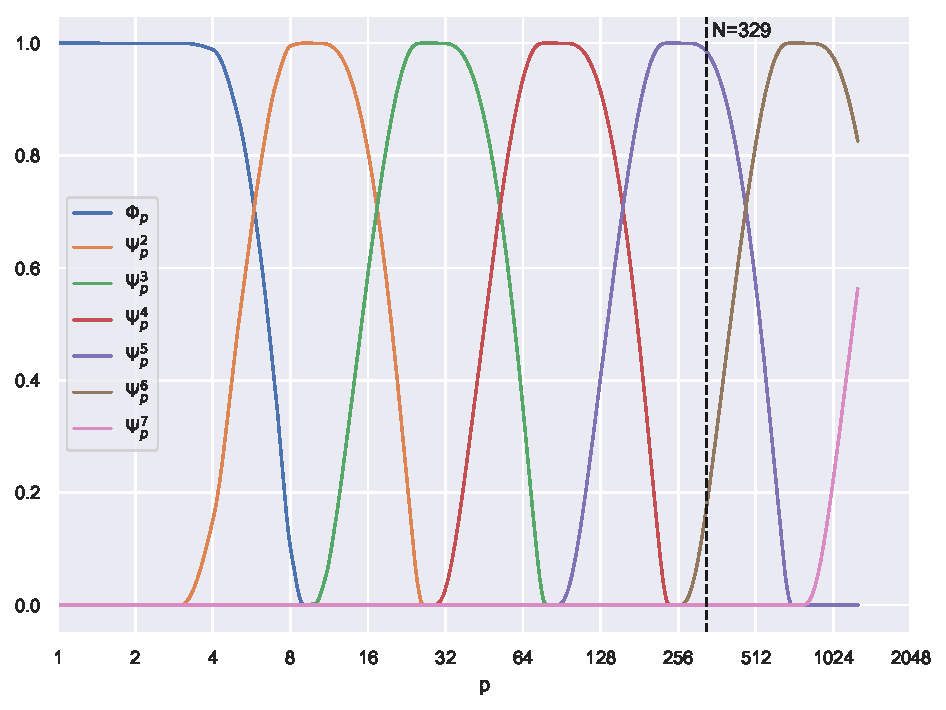
\includegraphics[width=\textwidth]{homer_slepian_tiling_b1275.pdf}
	\caption{
	}\label{fig:chapter4_tiling}
\end{figure}


\section{Numerical Illustration}

\begin{figure}[htp]
	\centering\capstart{}
	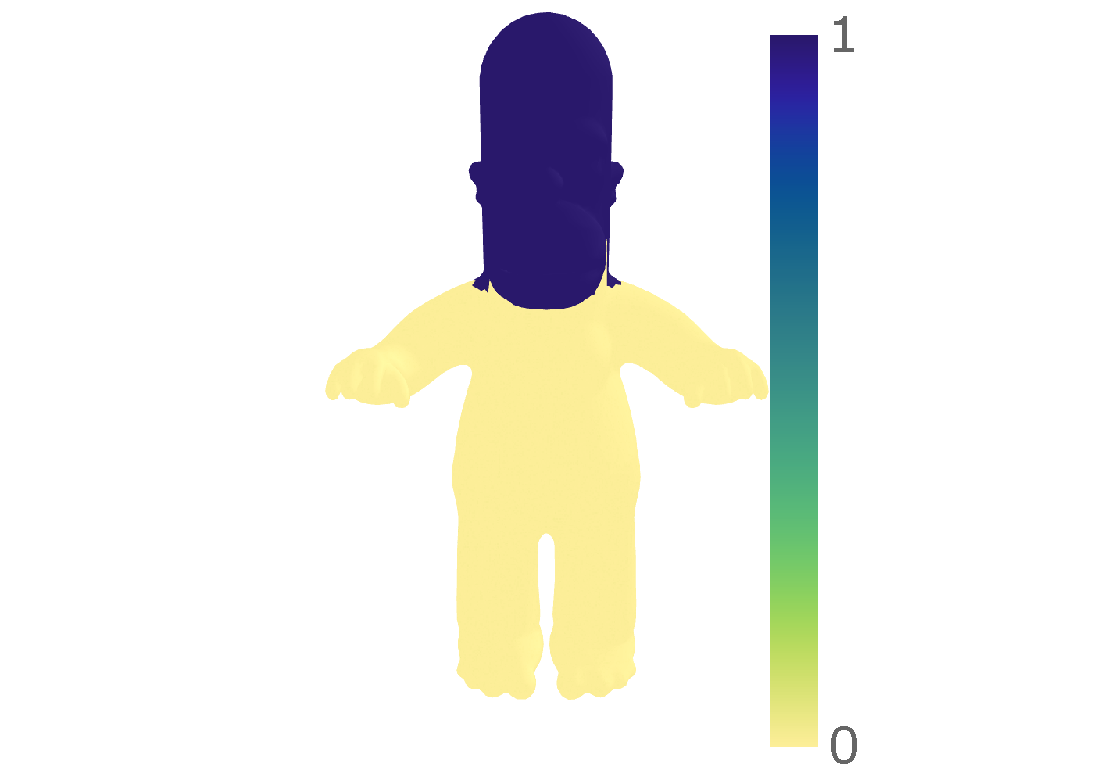
\includegraphics[trim={156 8 21 6},clip,width=.7\textwidth]{homer_region_norm.pdf}
	\caption[
		The head region of the Homer mesh
	]{
		The head region (in blue) chosen to compute the Slepian functions of the Homer mesh.
	}\label{fig:chapter4_homer_region}
\end{figure}


\begin{figure}[htp]
	\centering
	\subfloat[\(\mesh{S_{1}},\ \mu=1.00\)]
	{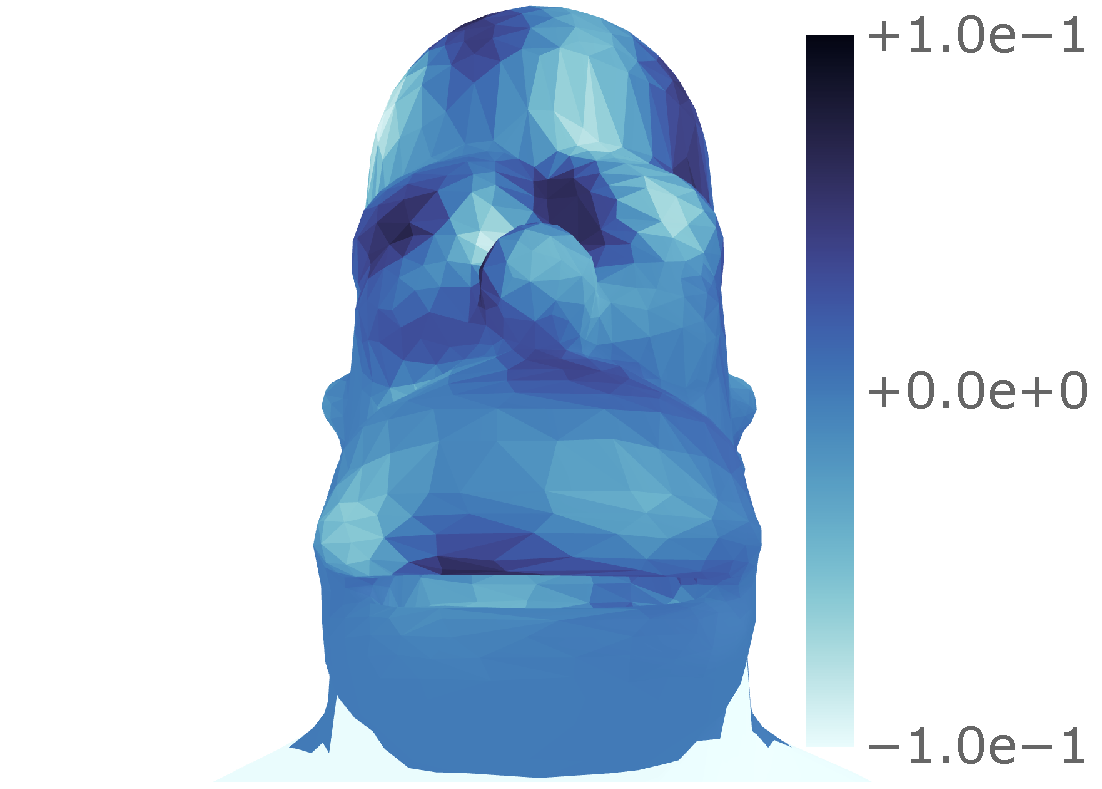
\includegraphics[trim={101 0 3 3},clip,width=.33\textwidth]{slepian_homer_rank0_lam1-000000e00_zoom.pdf}} % chktex 8
	\hfill
	\subfloat[\(\mesh{S_{10}},\ \mu=1.00\)]
	{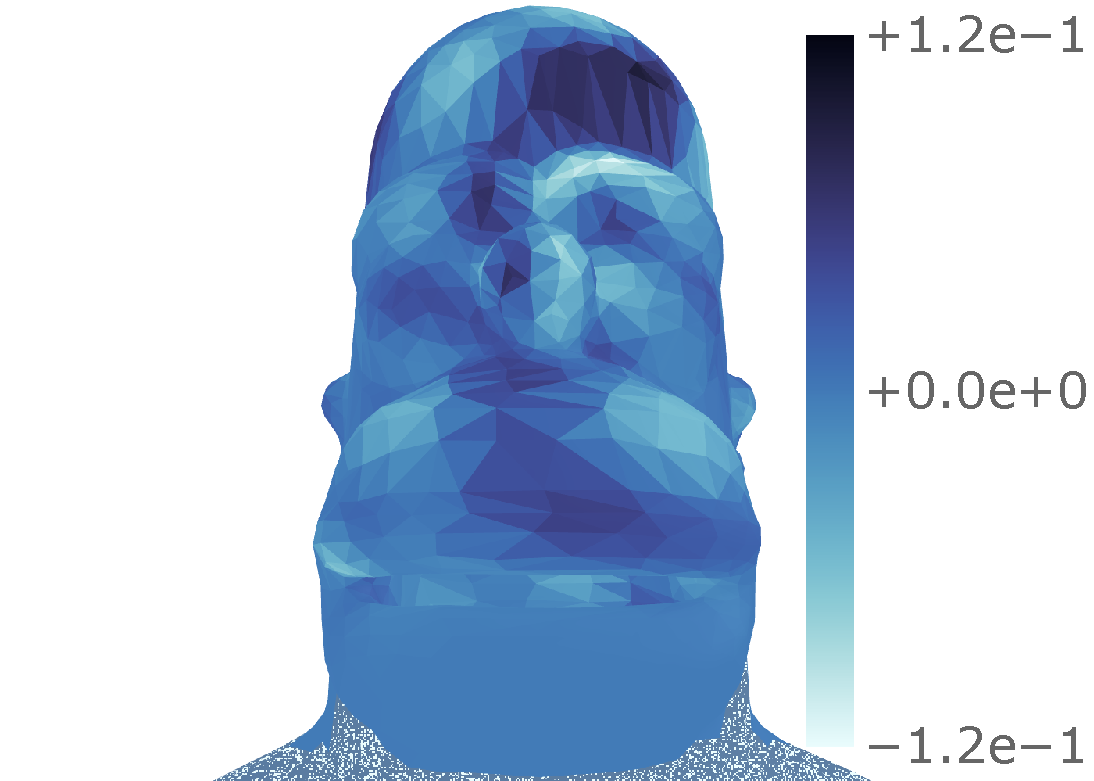
\includegraphics[trim={101 0 3 3},clip,width=.33\textwidth]{slepian_homer_rank9_lam1-000000e00_zoom.pdf}} % chktex 8
	\hfill
	\subfloat[\(\mesh{S_{25}},\ \mu=1.00\)]
	{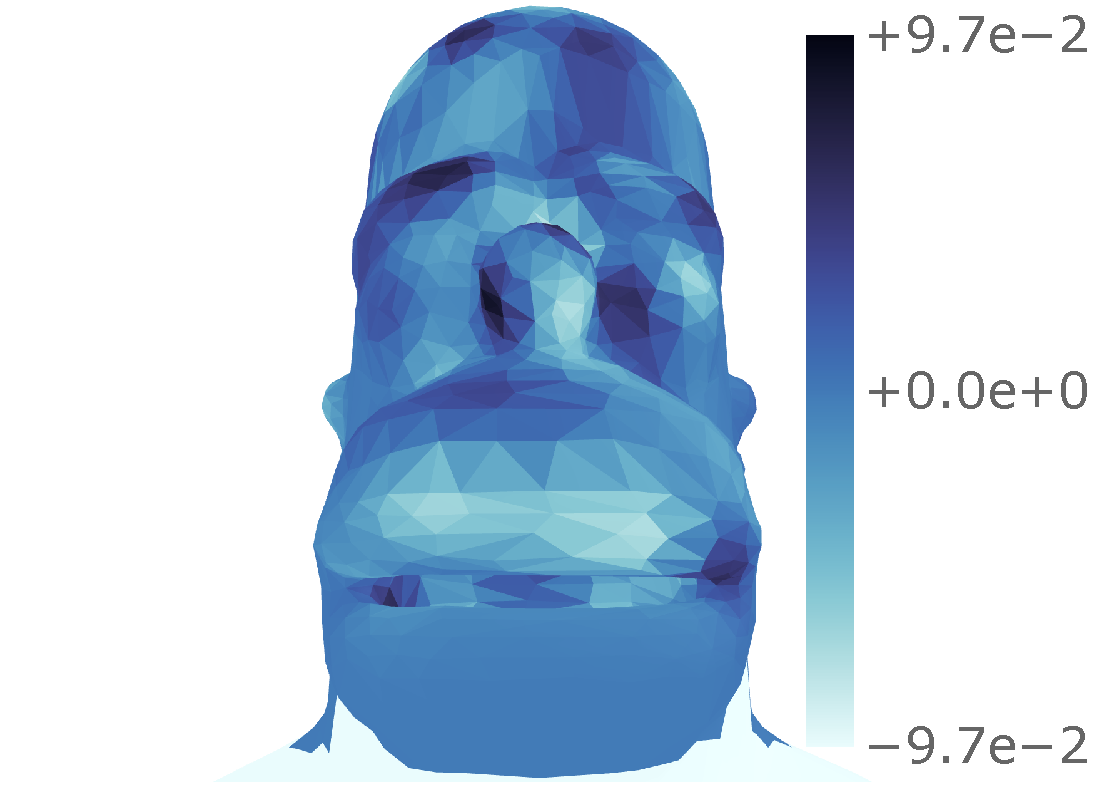
\includegraphics[trim={101 0 3 3},clip,width=.33\textwidth]{slepian_homer_rank24_lam1-000000e00_zoom.pdf}} % chktex 8
	\newline
	\subfloat[\(\mesh{S_{50}},\ \mu=1.00\)]
	{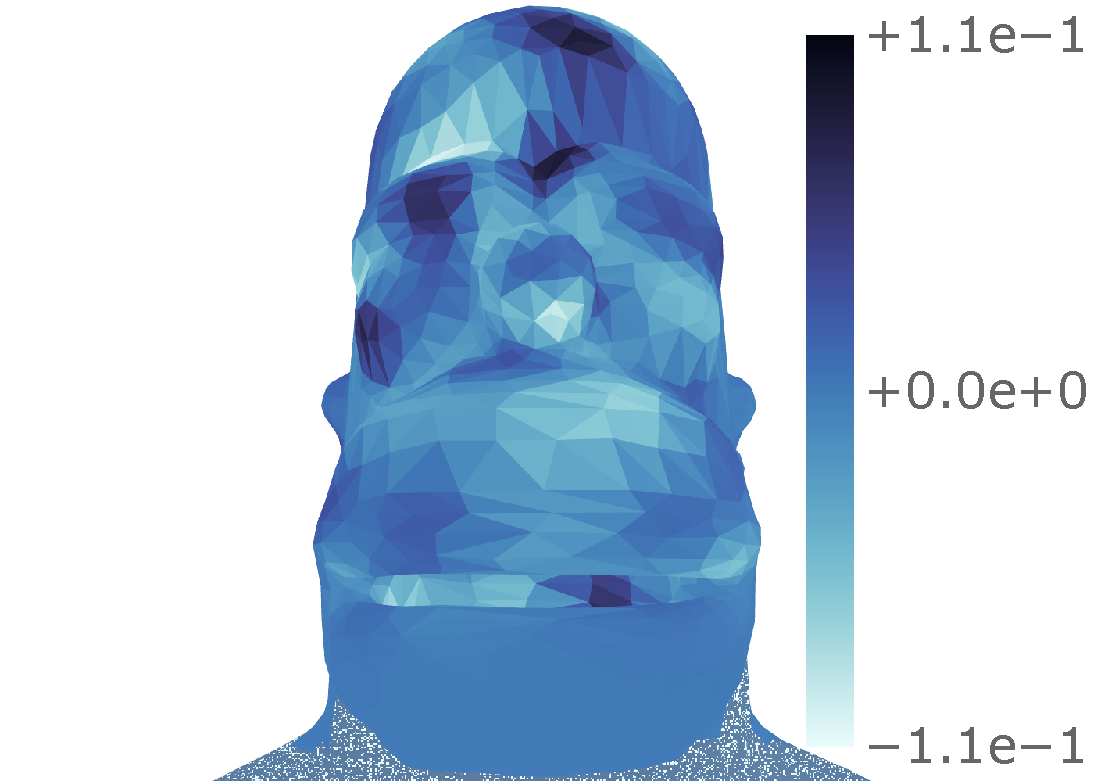
\includegraphics[trim={101 0 3 3},clip,width=.33\textwidth]{slepian_homer_rank49_lam1-000000e00_zoom.pdf}} % chktex 8
	\hfill
	\subfloat[\(\mesh{S_{100}},\ \mu=1.00\)]
	{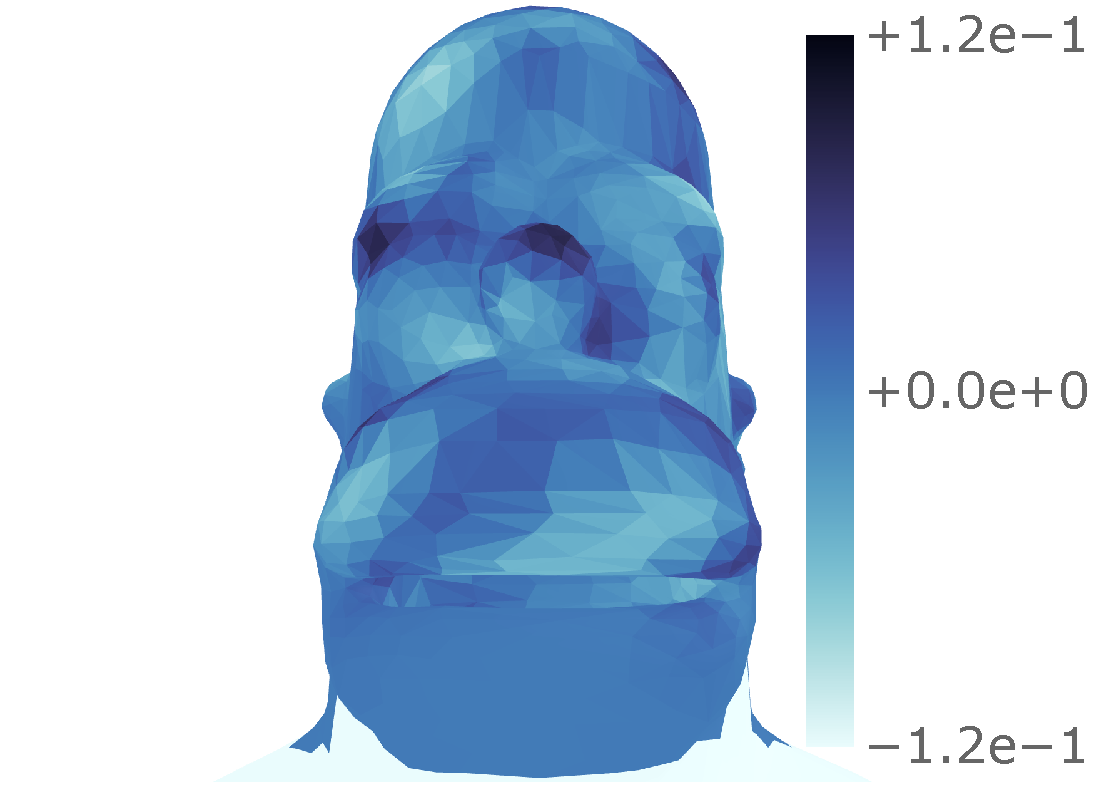
\includegraphics[trim={101 0 3 3},clip,width=.33\textwidth]{slepian_homer_rank99_lam1-000000e00_zoom.pdf}} % chktex 8
	\hfill
	\subfloat[\(\mesh{S_{200}},\ \mu=1.00\)]
	{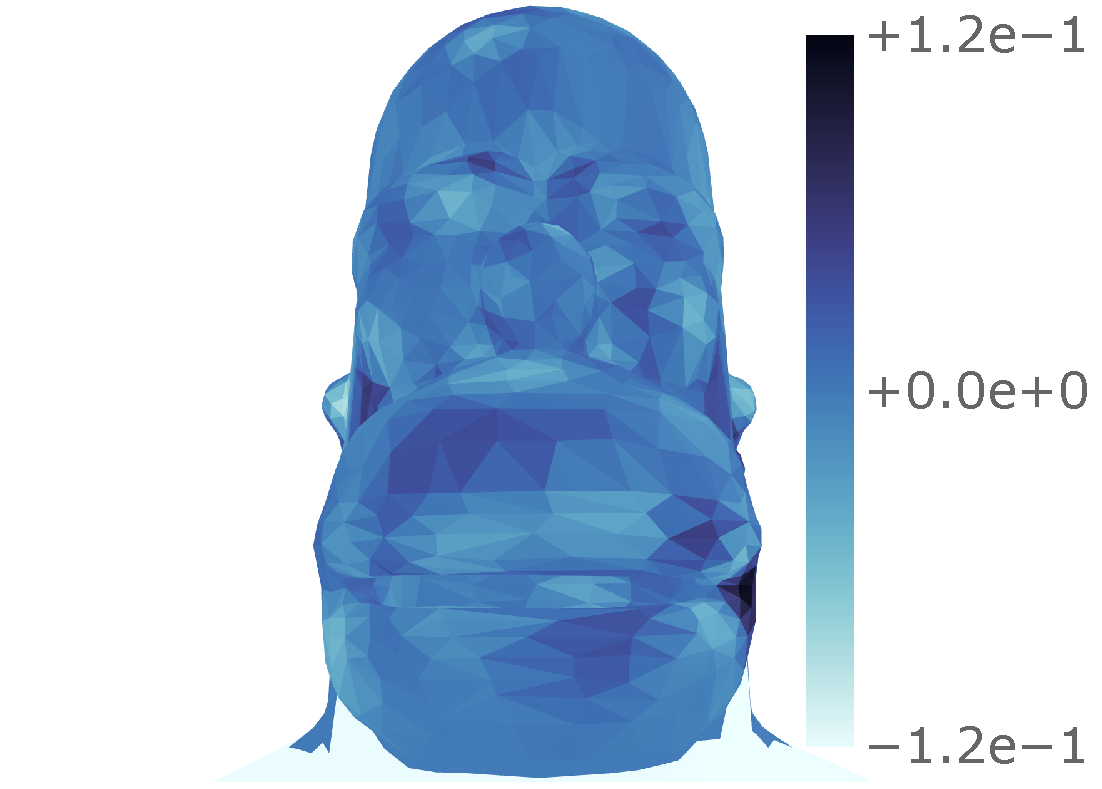
\includegraphics[trim={101 0 3 3},clip,width=.33\textwidth]{slepian_homer_rank199_lam1-000000e00_zoom.pdf}} % chktex 8
	\caption[
		Some Slepian functions of the Homer head region
	]{
		The Slepian functions of the Homer head region \(\mesh{\slepian{S}}\) for \(p \in \set{1, 10, 25, 50, 100, 200}\) shown left-to-right, top-to-bottom.
		The corresponding eigenvalue \(\slepian{\mu}\) is a measure of the concentration within the given region \(R\), which remains \(\almost{1}\) for many \(p\) values before decreasing towards zero.
		Whilst the Slepian functions are defined on the vertices, the values have been averaged onto the faces for the plot.
	}\label{fig:chapter4_slepian_functions}
\end{figure}


\begin{figure}[htp]
	\centering\capstart{}
	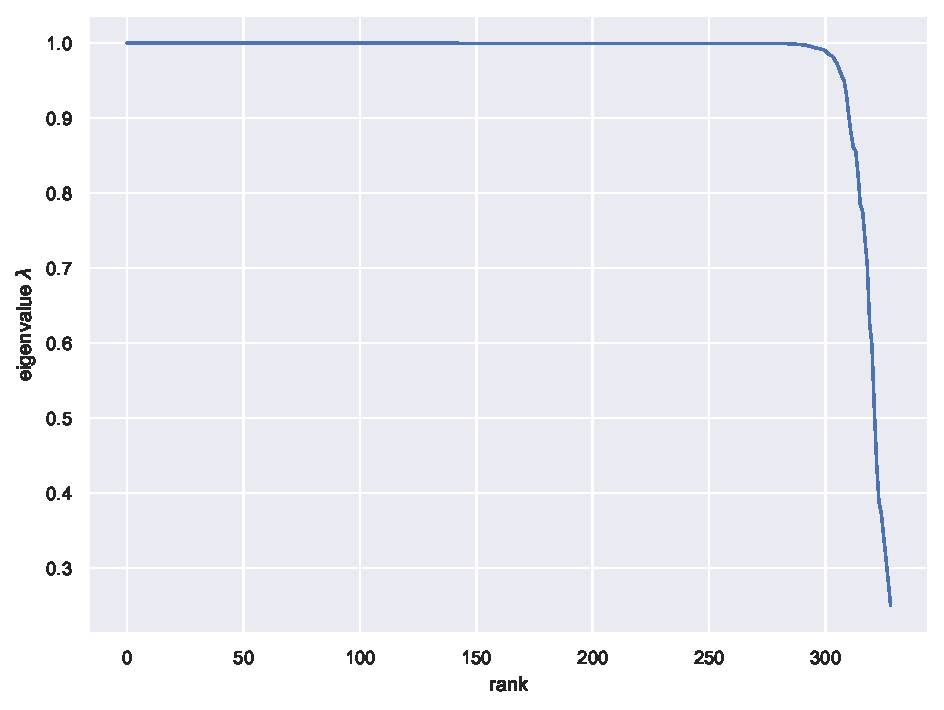
\includegraphics[width=\textwidth]{homer_slepian_eigenvalues_b1275.pdf}
	\caption[
		The Slepian eigenvalues of the Homer head region
	]{
		The eigenvalues of the Homer head region concentrated within the Shannon number \(N=329\).
		The majority of the eigenvalues are \(\almost{1}\) before decreasing rapidly towards zero around the Shannon number.
	}\label{fig:chapter4_slepian_eigenvalues}
\end{figure}


\begin{figure}[htpb]
	\centering\capstart{}
	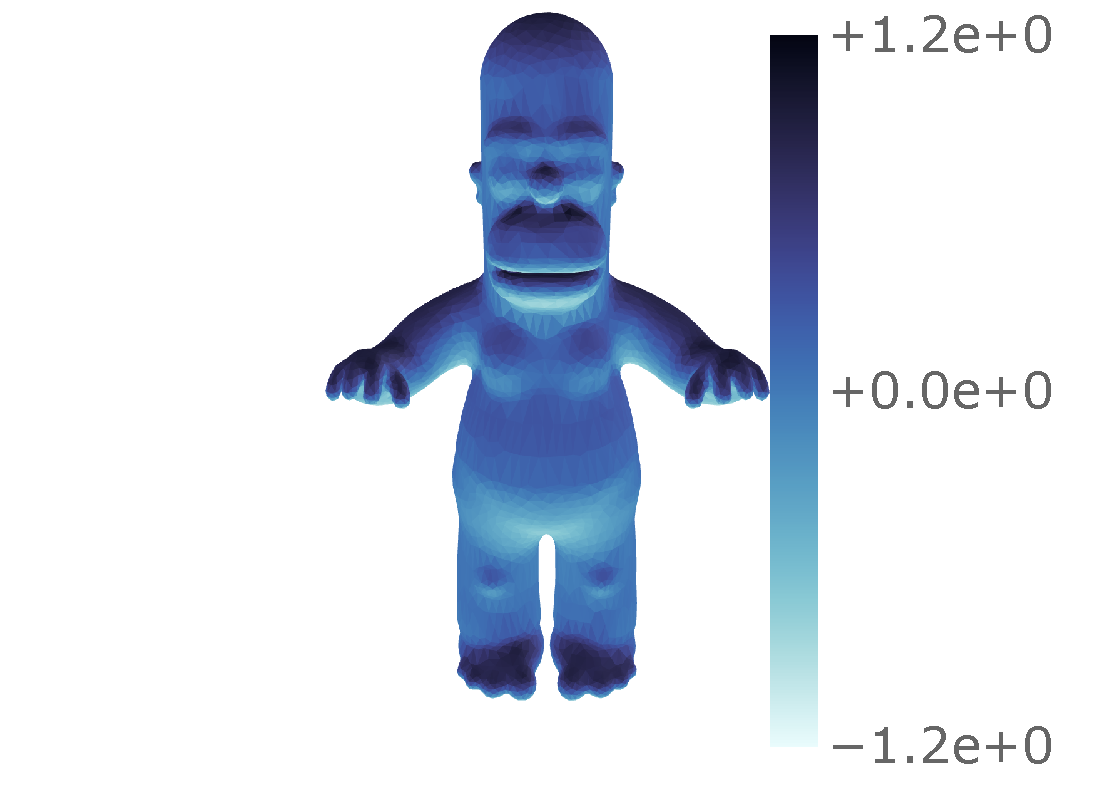
\includegraphics[trim={156 8 21 6},clip,width=.7\textwidth]{homer_field.pdf}
	\caption[
		An example field on the Homer mesh
	]{
		The \(z\)-component of the per vertex normals of the Homer mesh.
		Whilst the field is defined on the vertices, the values have been averaged onto the faces for the plot.
	}\label{fig:chapter4_homer_data}
\end{figure}


\begin{figure}[htp]
	\centering\capstart
	\subfloat[\(\mesh{\Phi}\)]
	{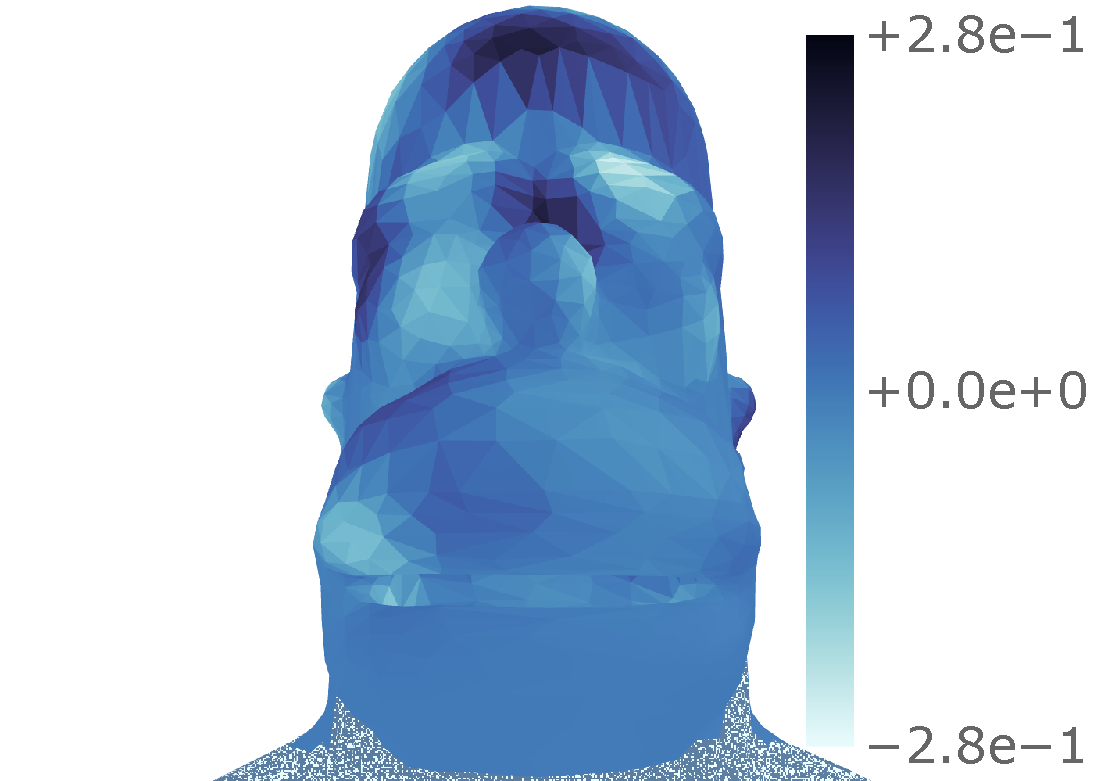
\includegraphics[trim={101 0 3 3},clip,width=.33\textwidth]{slepian_wavelets_homer_3B_2jmin_scaling_zoom.pdf}}
	\hfill
	\subfloat[\(\mesh{\Psi^{2j}}\)]
	{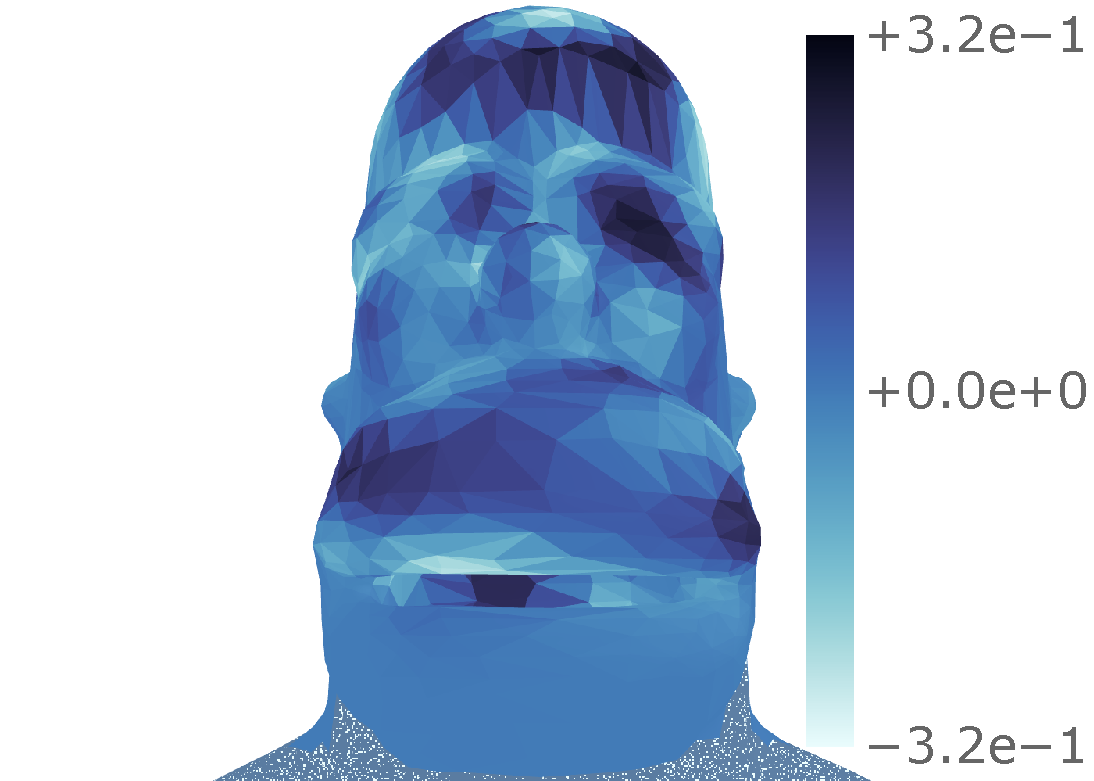
\includegraphics[trim={101 0 3 3},clip,width=.33\textwidth]{slepian_wavelets_homer_3B_2jmin_2j_zoom.pdf}}
	\hfill
	\subfloat[\(\mesh{\Psi^{3j}}\)]
	{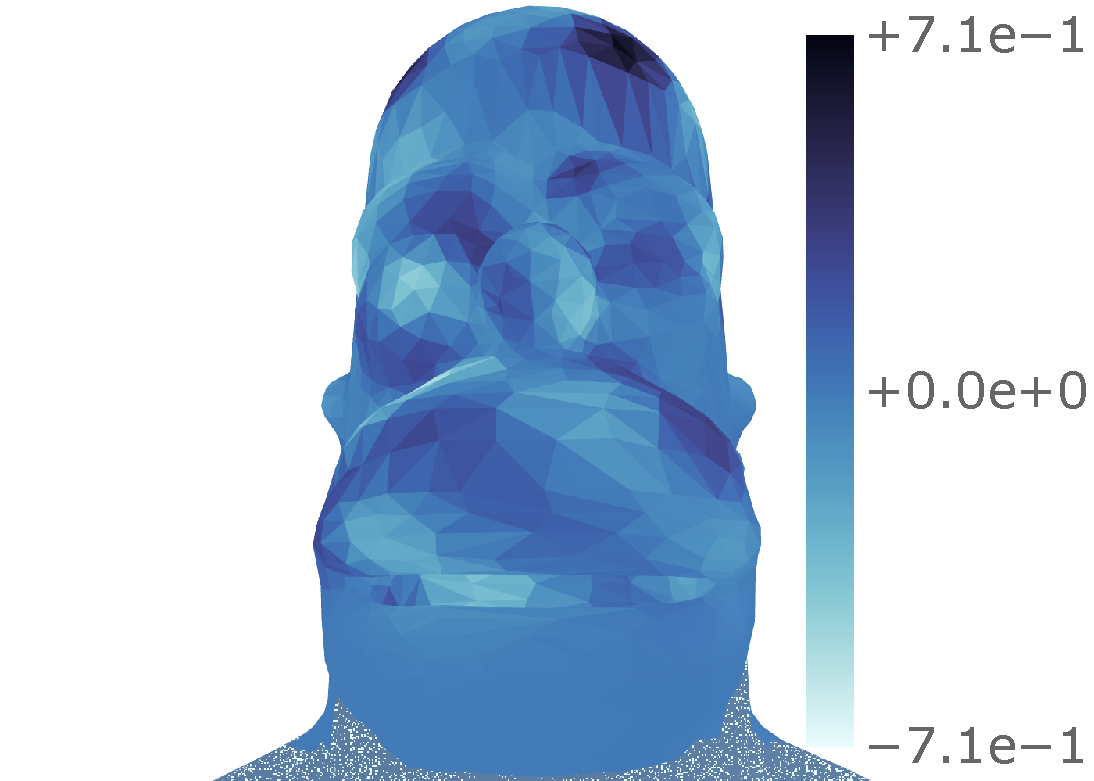
\includegraphics[trim={101 0 3 3},clip,width=.33\textwidth]{slepian_wavelets_homer_3B_2jmin_3j_zoom.pdf}}
	\newline
	\subfloat[\(\mesh{\Psi^{4j}}\)]
	{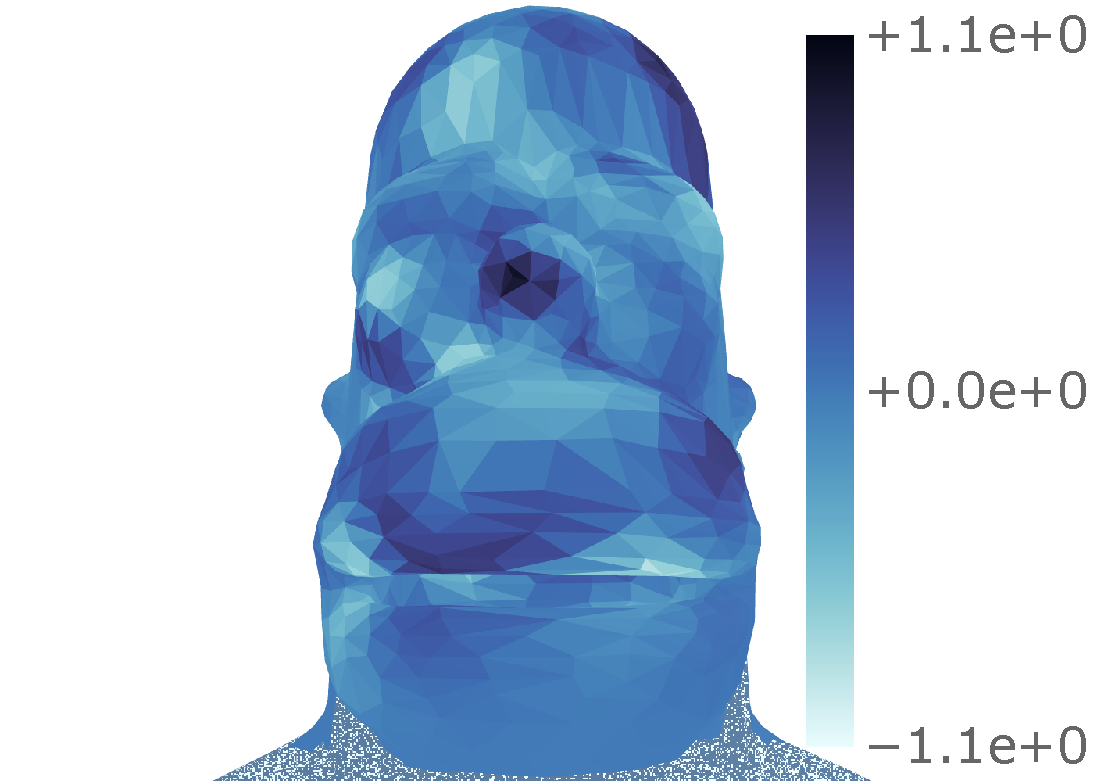
\includegraphics[trim={101 0 3 3},clip,width=.33\textwidth]{slepian_wavelets_homer_3B_2jmin_4j_zoom.pdf}}
	\hfill
	\subfloat[\(\mesh{\Psi^{5j}}\)]
	{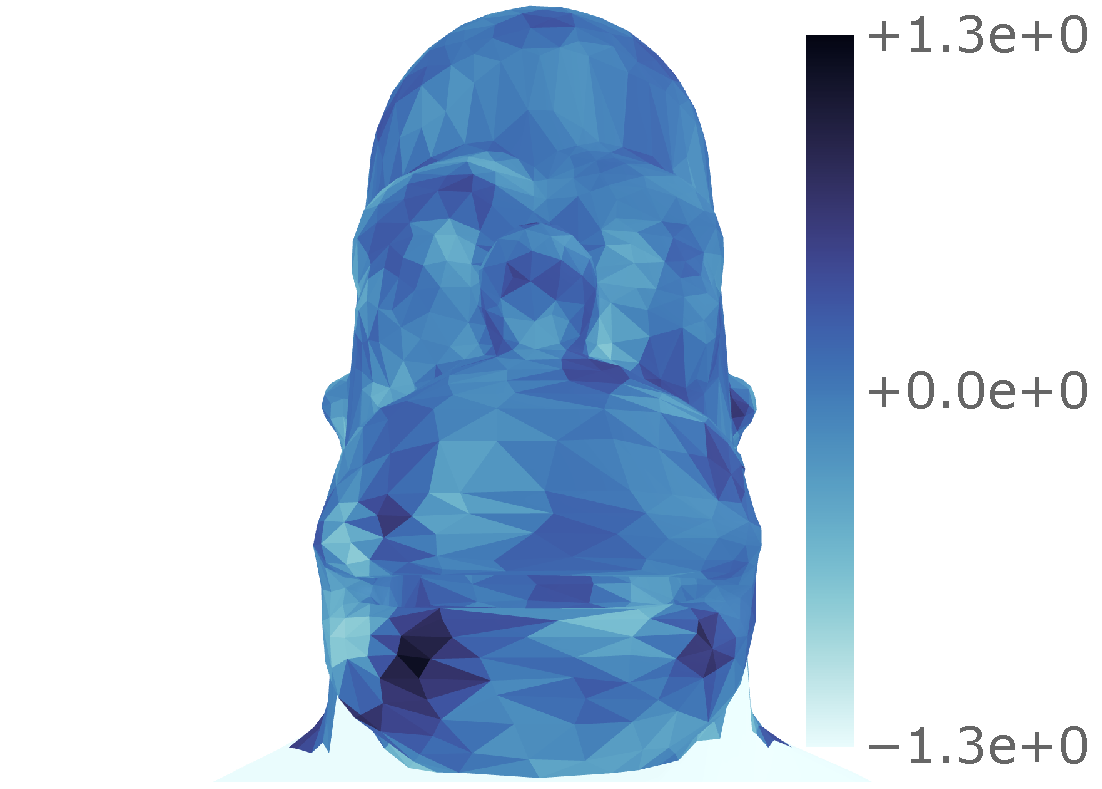
\includegraphics[trim={101 0 3 3},clip,width=.33\textwidth]{slepian_wavelets_homer_3B_2jmin_5j_zoom.pdf}}
	\hfill
	\subfloat[\(\mesh{\Psi^{6j}}\)]
	{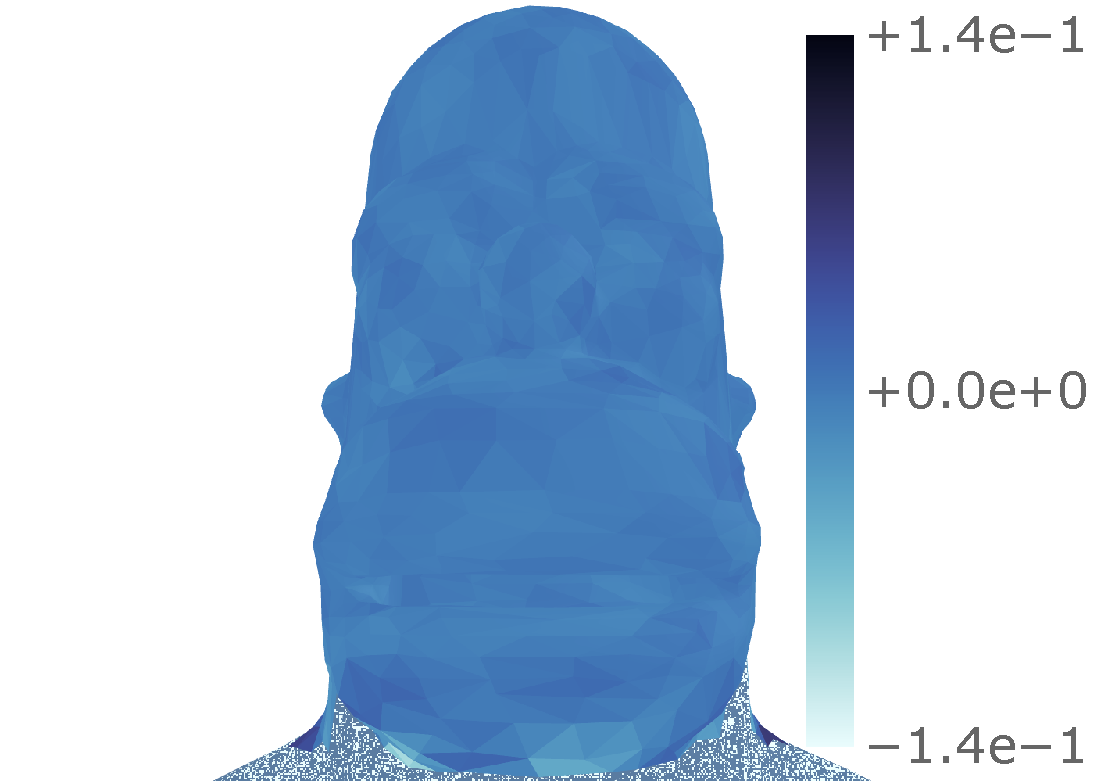
\includegraphics[trim={101 0 3 3},clip,width=.33\textwidth]{slepian_wavelets_homer_3B_2jmin_6j_zoom.pdf}}
	\caption[
		The Slepian wavelets of the Homer head region
	]{
		The scaling function and the wavelets for scales \(j \in \set{2, 3, 4, 5, 6}\) for the Homer head region shown left-to-right, top-to-bottom.
		The wavelets are constructed through a tiling of the Slepian line using scale-discretised functions, with parameters \(\lambda=3\), \(J_{0}=2\), and \(\imax=\num{1275}\) basis functions.
		Whilst the wavelets are defined on the vertices, the values have been averaged onto the faces for the plot.
	}\label{fig:chapter4_wavelets}
\end{figure}


\begin{figure}[htp]
	\centering
	\subfloat[\(\mesh{W^{\Phi}}\)]
	{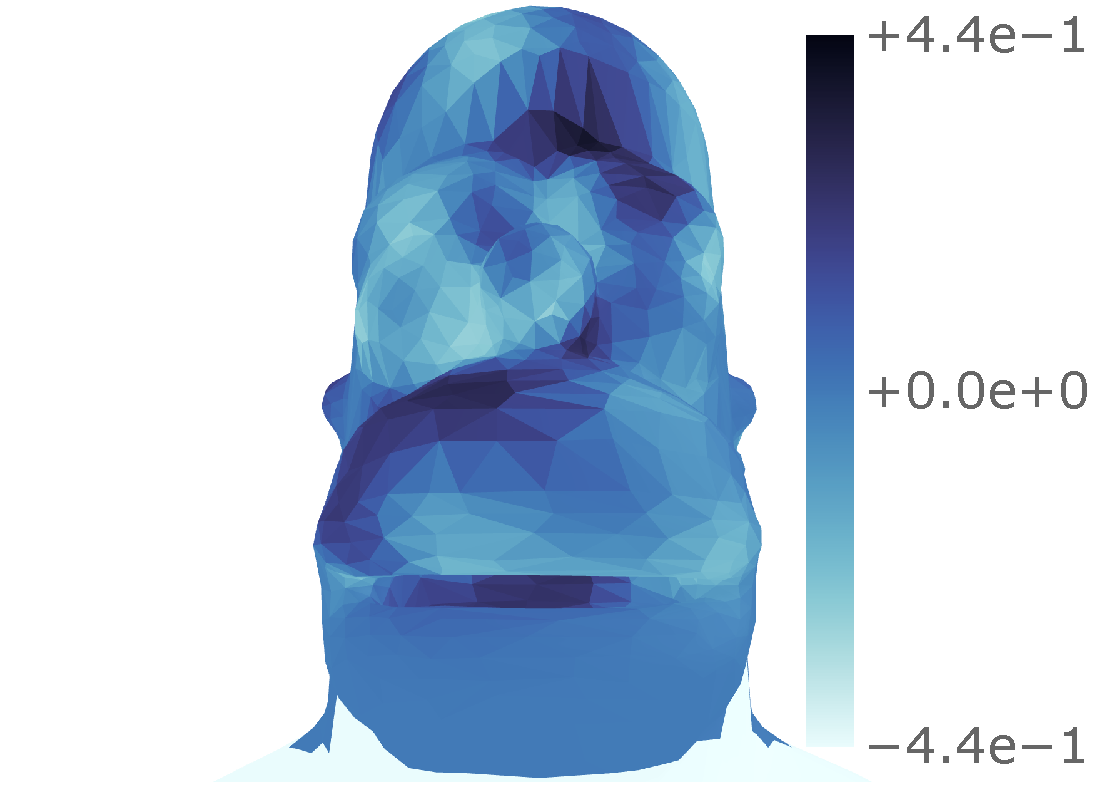
\includegraphics[trim={101 0 3 3},clip,width=.33\textwidth]{slepian_wavelet_coefficients_homer_3B_2jmin_scaling_zoom.pdf}}
	\hfill
	\subfloat[\(\mesh{W^{\Psi^{2j}}}\)]
	{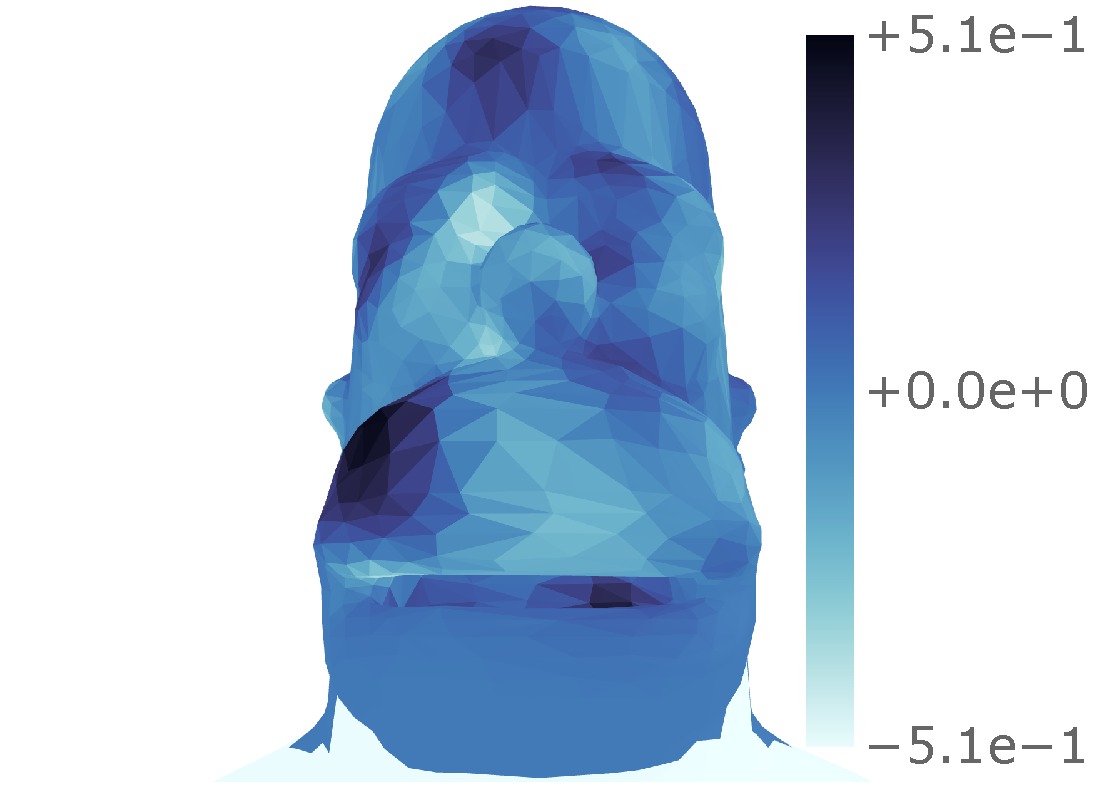
\includegraphics[trim={101 0 3 3},clip,width=.33\textwidth]{slepian_wavelet_coefficients_homer_3B_2jmin_2j_zoom.pdf}}
	\hfill
	\subfloat[\(\mesh{W^{\Psi^{3j}}}\)]
	{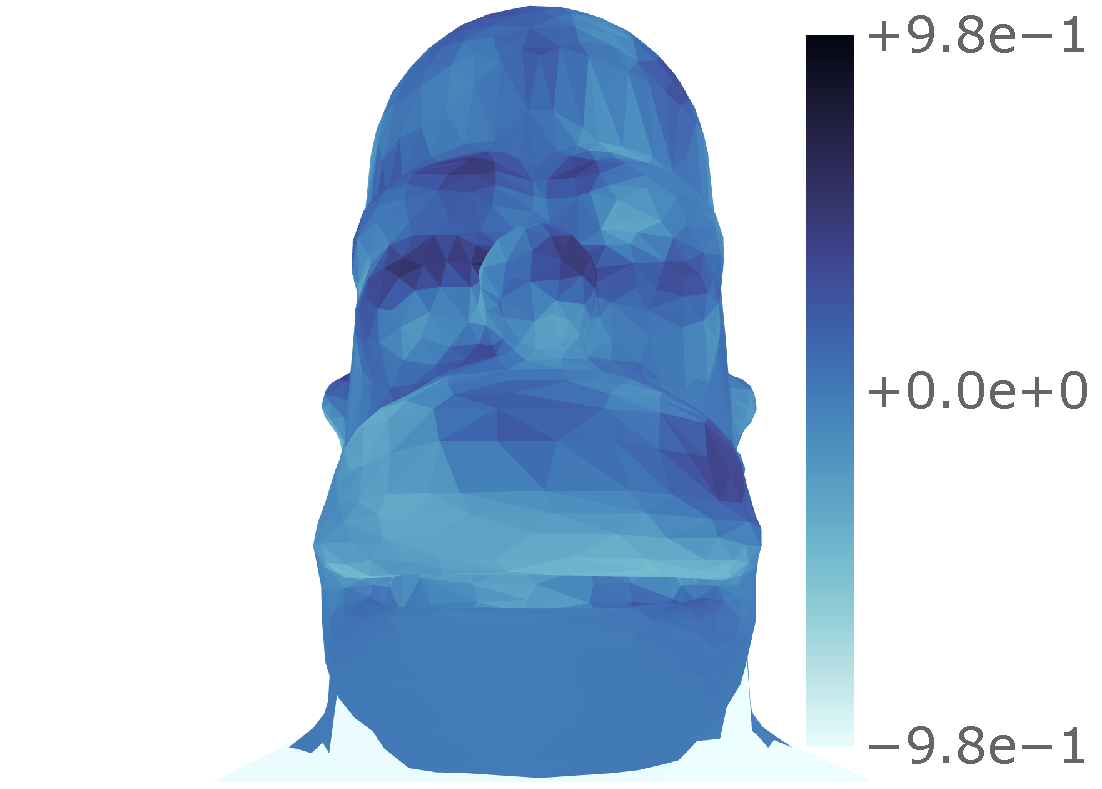
\includegraphics[trim={101 0 3 3},clip,width=.33\textwidth]{slepian_wavelet_coefficients_homer_3B_2jmin_3j_zoom.pdf}}
	\newline
	\subfloat[\(\mesh{W^{\Psi^{4j}}}\)]
	{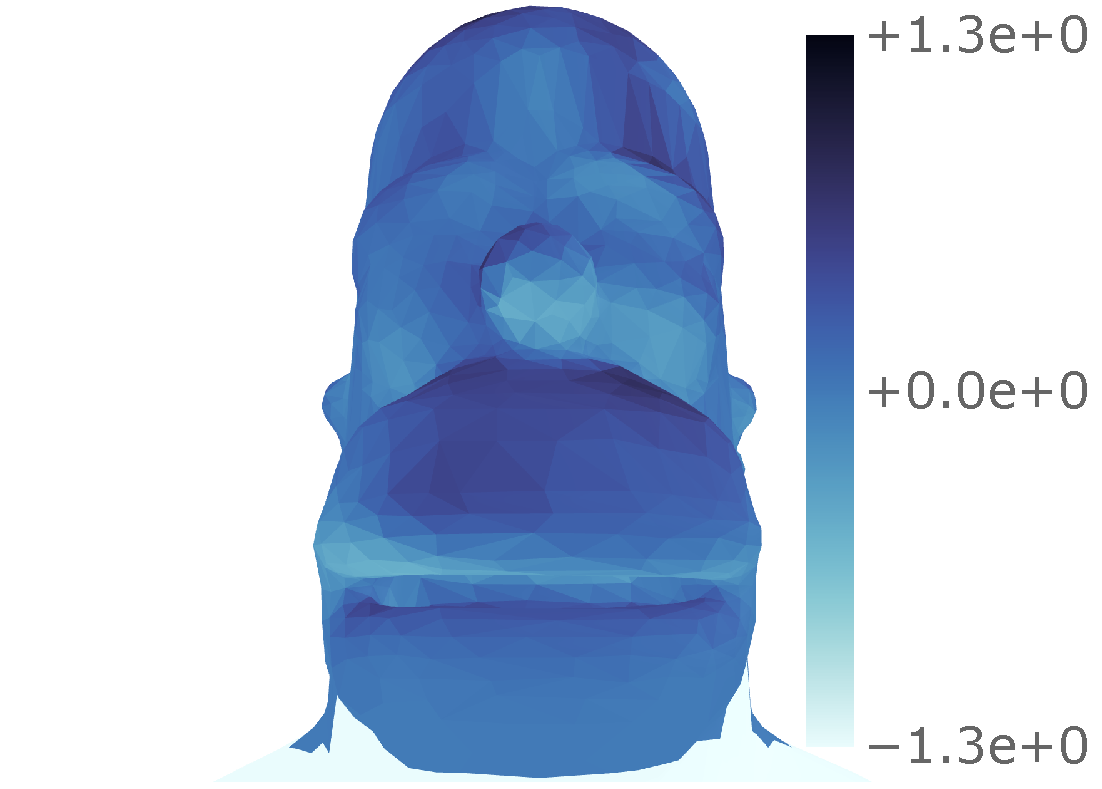
\includegraphics[trim={101 0 3 3},clip,width=.33\textwidth]{slepian_wavelet_coefficients_homer_3B_2jmin_4j_zoom.pdf}}
	\hfill
	\subfloat[\(\mesh{W^{\Psi^{5j}}}\)]
	{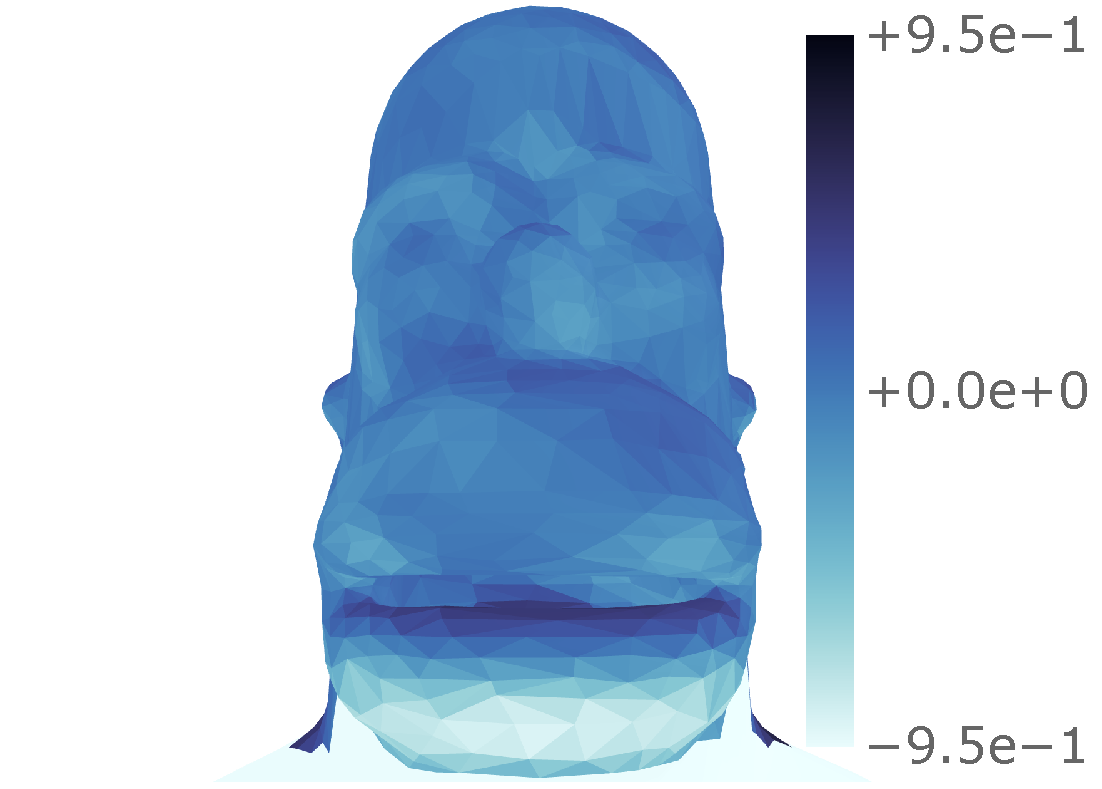
\includegraphics[trim={101 0 3 3},clip,width=.33\textwidth]{slepian_wavelet_coefficients_homer_3B_2jmin_5j_zoom.pdf}}
	\hfill
	\subfloat[\(\mesh{W^{\Psi^{6j}}}\)]
	{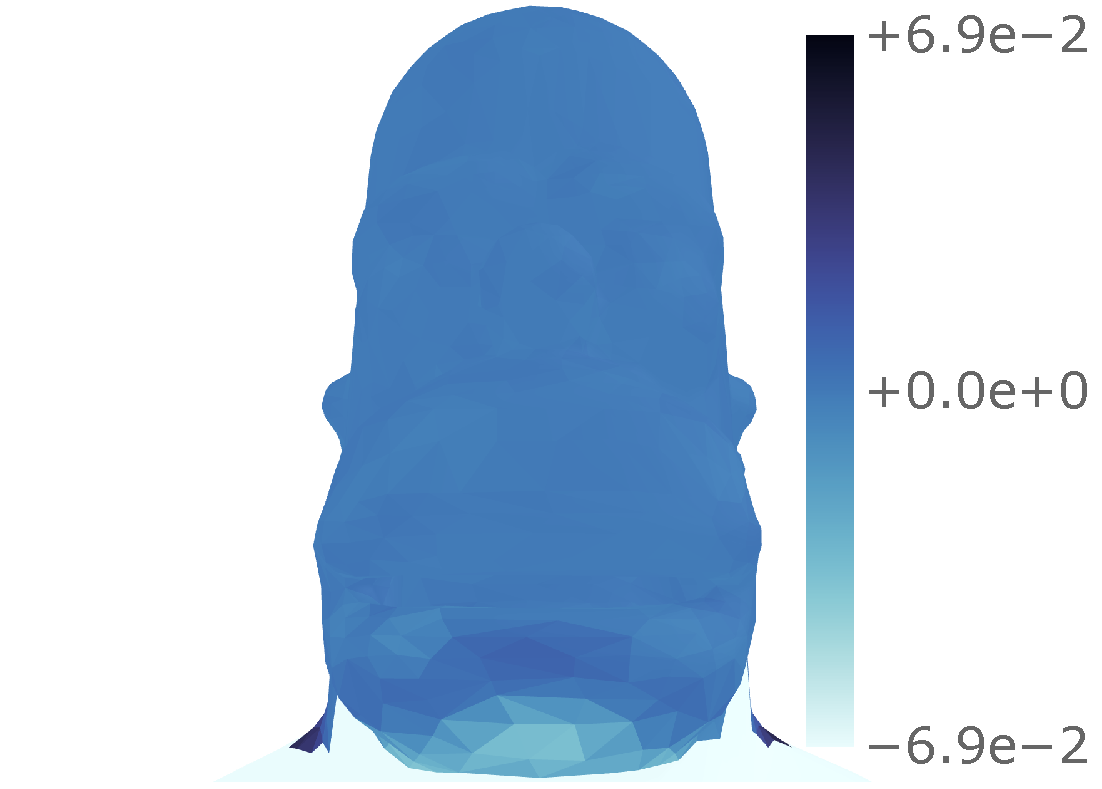
\includegraphics[trim={101 0 3 3},clip,width=.33\textwidth]{slepian_wavelet_coefficients_homer_3B_2jmin_6j_zoom.pdf}}
	\caption{
	}\label{fig:chapter4_wavelet_coefficients}
\end{figure}


\begin{figure}[htp]
	\centering\capstart{}
	\subfloat[Initial Data]
	{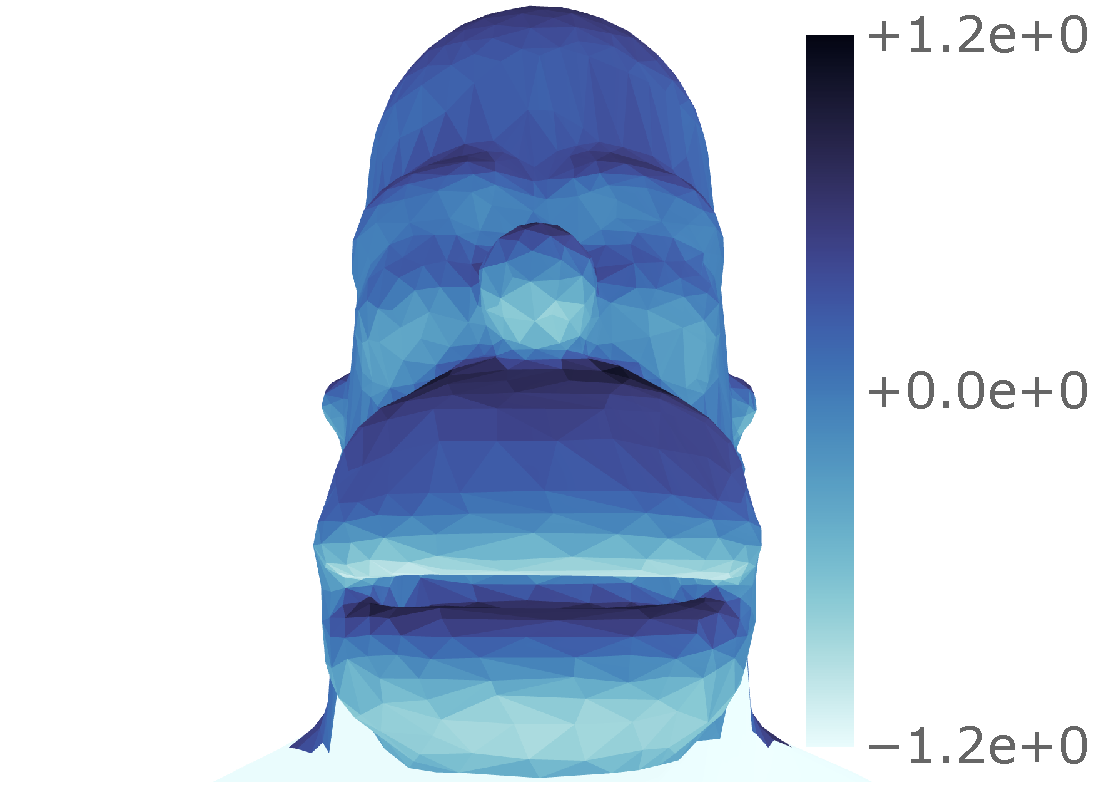
\includegraphics[trim={101 0 3 3},clip,width=.33\textwidth]{slepian_homer_field_zoom.pdf}}
	\hfill
	\subfloat[Noisy Data \newline
		\(\snr{z} = \SI{0.32}{\dB}\)]
	{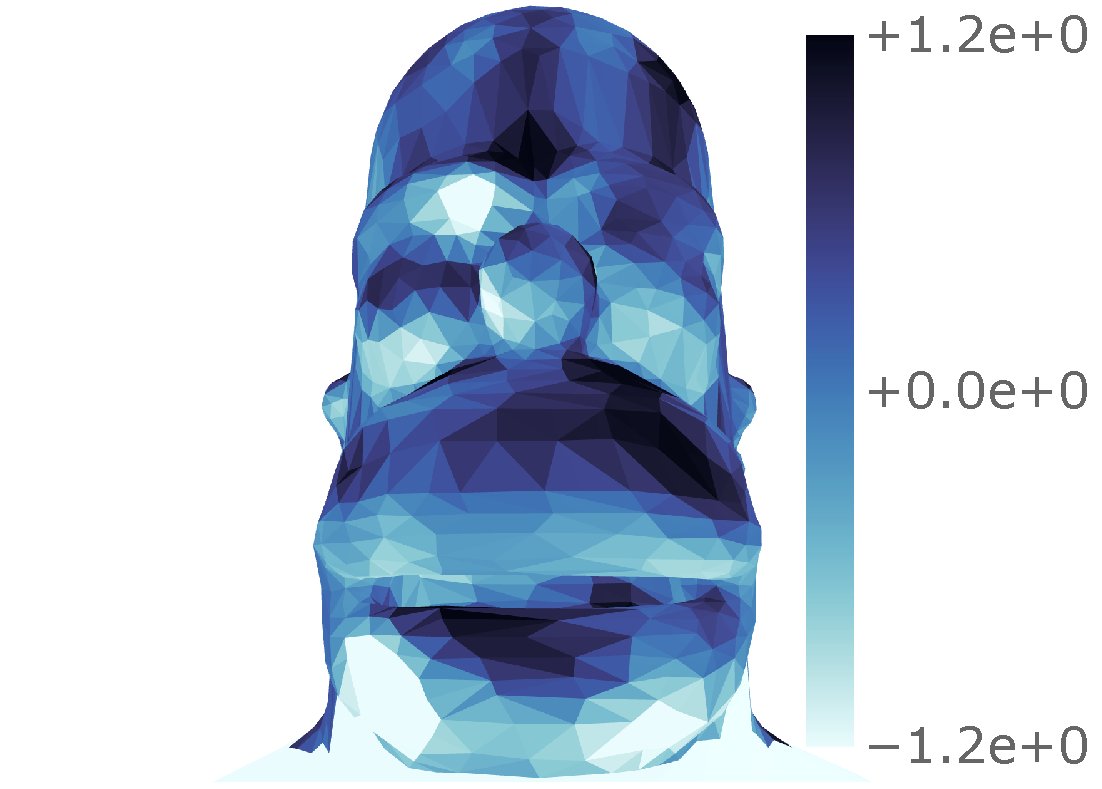
\includegraphics[trim={101 0 3 3},clip,width=.33\textwidth]{slepian_homer_field_-5noise_zoom.pdf}}
	\hfill
	\subfloat[Denoised \(N_{\sigma}=1\) \newline
		\(\snr{d} = \SI{2.29}{\dB}\)]
	{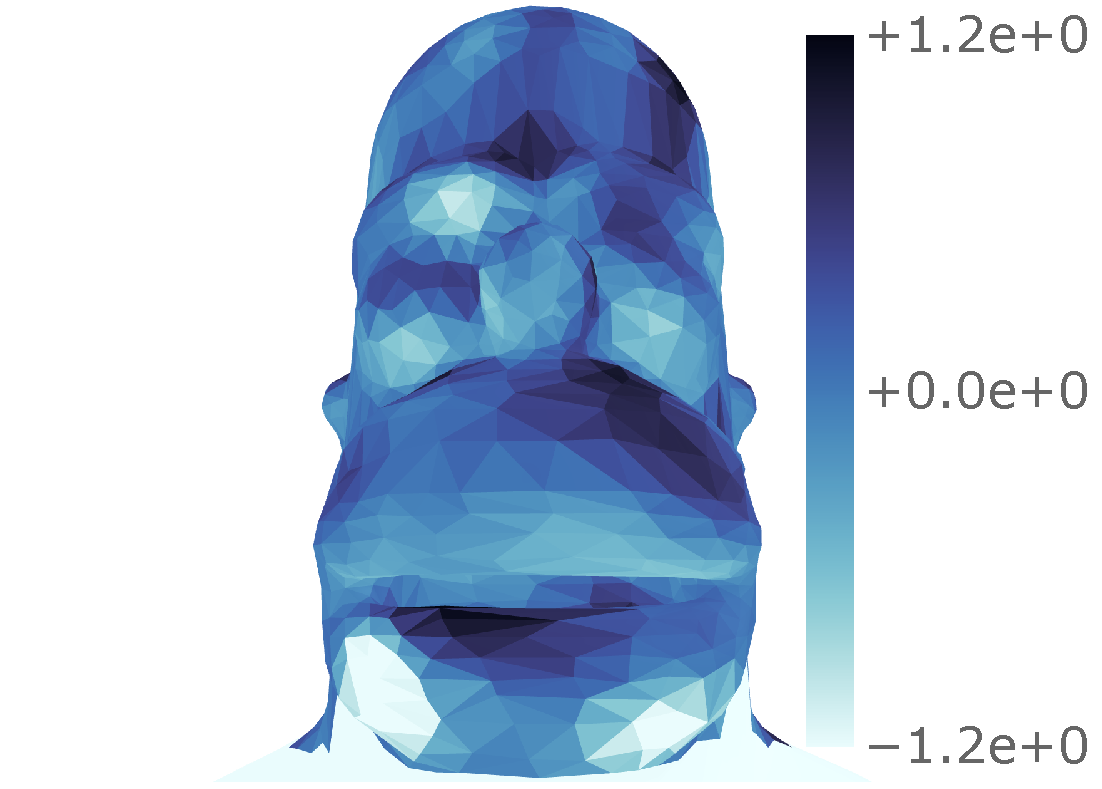
\includegraphics[trim={101 0 3 3},clip,width=.33\textwidth]{homer_-5snr_1n_denoised.pdf}}
	\caption[
		A denoising demonstration for a field on the Homer mesh
	]{
		Panel (a) shows the data in the region \(R\) constructed from the Slepian coefficients of the per vertex normals (\cf{} \cref{fig:chapter4_homer_data}) --- where the field value outside the region is set to negative infinity for illustrative purposes.
		Gaussian white noise is added to the signal in the Homer head region with a signal-to-noise ratio of \(\SI{0.32}{\dB}\), shown in panel (b).
		The scaling and wavelet coefficients of the noisy signal are calculated and are then hard-thresholded with \(N_{\sigma}=1\).
		The corresponding denoised plot is shown in panel (c), where the signal-to-noise ratio is boosted by \(\SI{1.97}{\dB}\) to \(\SI{2.29}{\dB}\).
		Whilst the signal values are defined on the vertices, they have been averaged onto the faces for the plot.
	}\label{fig:chapter4_denoising}
\end{figure}


\begin{figure}[htp]
	\centering
	\subfloat[Bird]
	{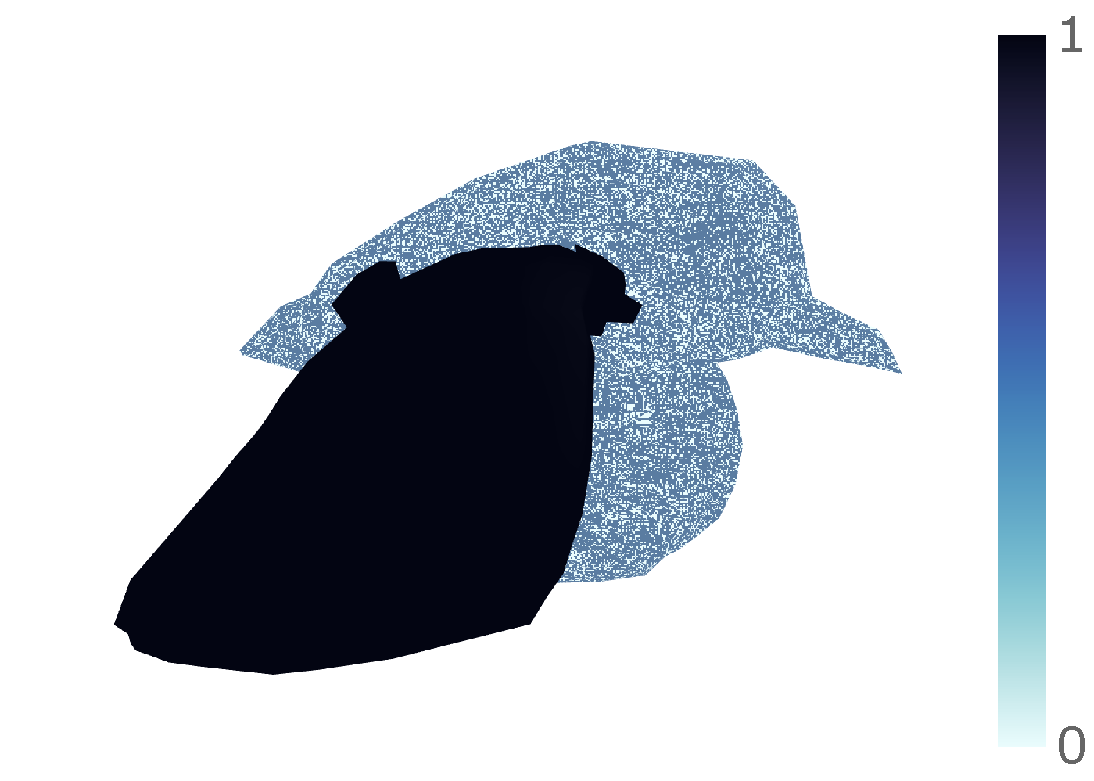
\includegraphics[trim={7 8 3 7},clip,width=.38\textwidth]{bird_region_norm.pdf}}
	\hfill
	\subfloat[Cheetah]
	{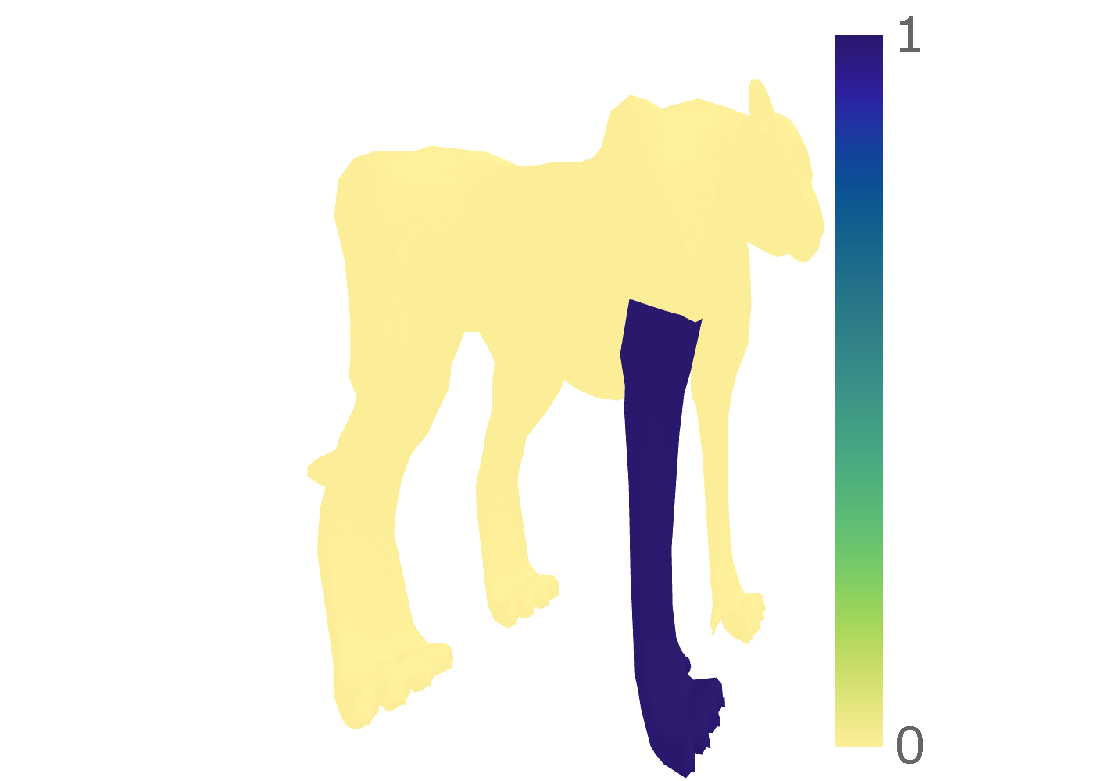
\includegraphics[trim={137 1 3 7},clip,width=.28\textwidth]{cheetah_region_norm.pdf}}
	\hfill
	\subfloat[Cube]
	{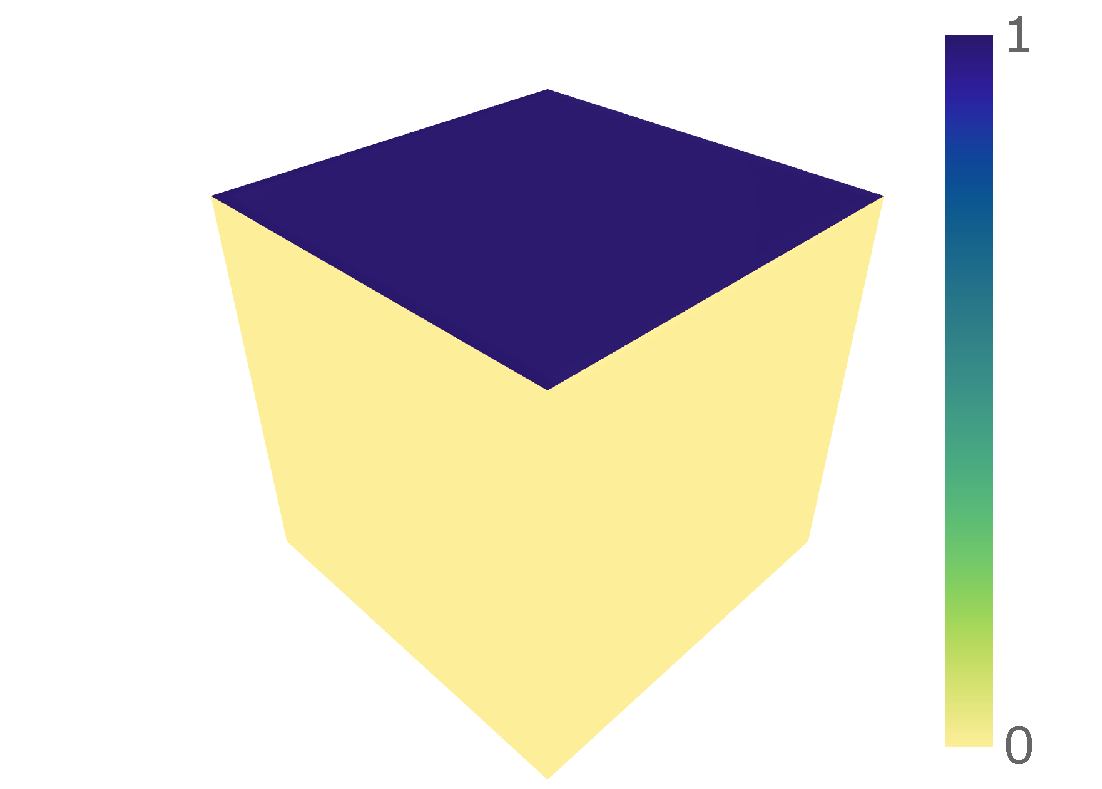
\includegraphics[trim={62 1 3 7},clip,width=.33\textwidth]{cube_region_norm.pdf}}
	\newline
	\subfloat[Dragon]
	{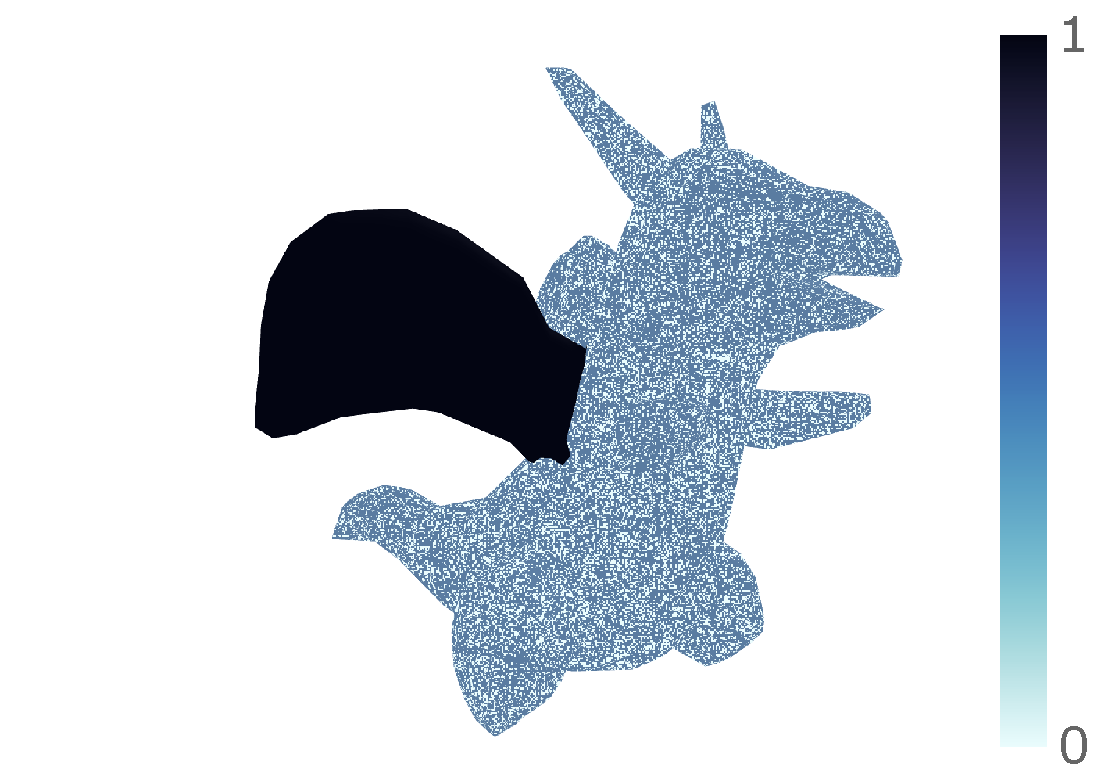
\includegraphics[trim={75 8 3 7},clip,width=.33\textwidth]{dragon_region_norm.pdf}}
	%
	\subfloat[Teapot]
	{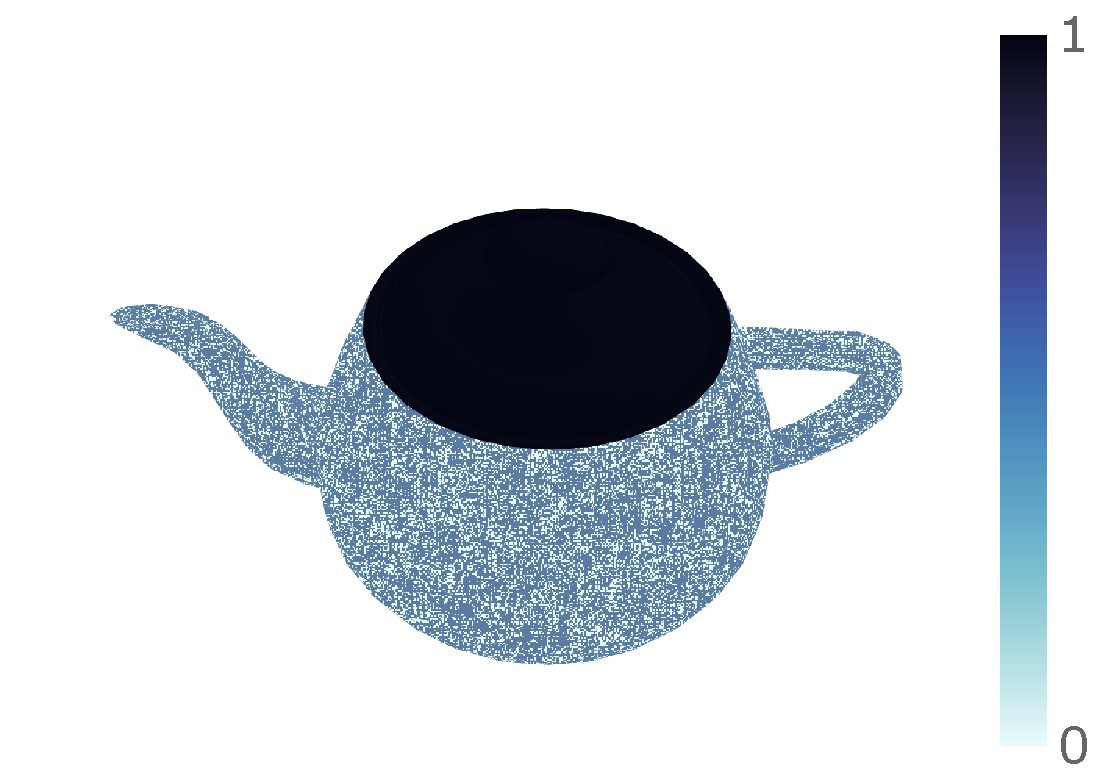
\includegraphics[trim={3 8 3 7},clip,width=.38\textwidth]{teapot_region_norm.pdf}}
	\caption{
		The Slepian regions (in black) of some other meshes.
		The same denoising procedure as in \cref{fig:chapter4_denoising} was performed for these alternative meshes, the results are shown in \cref{tab:chapter4_denoising}.
	}\label{fig:chapter4_other_meshes}
\end{figure}


\begin{table}
	\centering
	\caption{
		Denoising of other meshes.
	}\label{tab:chapter4_denoising}
	\begin{tabular}{@{}rcccc@{}}
		\toprule
		        & Shannon       & Wavelets    & Initial SNR         & \(N_{\sigma}=1\) SNR \\
		\midrule
		Cheetah & \(\num{72}\)  & \(\num{4}\) & \(\SI{3.96}{\dB}\)  & \(\SI{3.58}{\dB}\)   \\
		%
		Dragon  & \(\num{169}\) & \(\num{5}\) & \(\SI{3.44}{\dB}\)  & \(\SI{2.69}{\dB}\)   \\
		%
		Bird    & \(\num{194}\) & \(\num{5}\) & \(\SI{0.49}{\dB}\)  & \(\SI{1.59}{\dB}\)   \\
		%
		Teapot  & \(\num{256}\) & \(\num{6}\) & \(\SI{-1.57}{\dB}\) & \(\SI{-0.08}{\dB}\)  \\
		%
		Cube    & \(\num{272}\) & \(\num{6}\) & \(\SI{2.65}{\dB}\)  & \(\SI{3.85}{\dB}\)   \\
		%
		Homer   & \(\num{329}\) & \(\num{6}\) & \(\SI{0.32}{\dB}\)  & \(\SI{2.29}{\dB}\)   \\
		\bottomrule
	\end{tabular}
\end{table}

